\newpage

% Из текста короткого задания на ВКР:
% 1. Определение средств разработки и архитектуры системы: разработка ее структуры;
% 2. определение набора необходимого оборудования, программного обеспечения.

% 3. Проектирование и определение спецификаций аппаратной и программной компонентов системы.
% 4. Реализация компонентов системы с использованием выбранных средств разработки.
% 5. Сборка макета аппаратной подсистемы.
% 6. Сборка, установка и тестирование программного обеспечения аппаратной и программных подсистем.
% 7. Тестирования системы, интеграции программной и аппаратных частей.

\section{Разработка программно-аппаратной системы}

В данном разделе описывается проектирование аппаратной части системы~--- считывателя бесконтактных платежных карт~--- и разработка программной части СБО~--- программного обеспечения для считывателя и мобильного приложение бесконтактной оплаты.
Для этого в соответствии с техническим заданием (ТЗ) решаются следующие задачи:

\begin{itemize}
    \item определение средств разработки и архитектуры системы: разработка ее структуры; определение набора необходимого оборудования, программного обеспечения;
    \item проектирование компонентов и определение спецификаций аппаратной части СБО, сборка макета аппаратной части системы;
    \item выбор архитектуры и подхода разработки программной подсистемы, проектирование программных компонентов СБО (программы мобильного терминала бесконтактной оплаты и мобильного приложения оплаты) и определение спецификаций компонентов;
    \item реализация компонентов системы с использованием выбранных средств разработки;
    \item сборка, установка и тестирование программного обеспечения аппаратной подсистемы и программного обеспечения программной подсистемы.
\end{itemize}

Разрабатываемая система является mPOS-терминалом с поддержкой бесконтактной оплаты.
Как любой mPOS-терминал она состоит из мобильного устройства и считывателя платежных карт, подключаемого к ней.
В соответствии с требованиями ТЗ считыватель поддерживает только бесконтактные карты и подключается беспроводным образов посредством технологии Bluetooth.
Считыватель взаимодействует с платежным средством посредством технологии NFC.

Процесс оплаты с использованием устройства представляет следующую последовательность действия:
\begin{enumerate}
    \item представить торгово-сервисного предприятия (ТСП) вводит данные о платеже в мобильное приложение и активирует считыватель;
    \item держатель карты прикладывает к считывателю средства платежа (карта или мобильное приложение, эмулирующее платежную карту);
    \item считыватель взаимодействует со средством платежа и передает данные, необходимые для формирования платежа, на мобильное устройство;
    \item мобильное устройство отправляет HTTP-запрос на сервер банка-эквайера для выполнения платежа;
    \item сервер банка-эквайера отправляет HTTP-ответ на мобильное устройство, сообщая о статусе операции.
\end{enumerate}

Плательщик (держатель карты) может убрать средство платежа от считывателя после того как считыватель выполнит все необходимые операции для получения данных, необходимых для формирования платежа, либо сообщит о невозможности продолжения транзакции из-за ошибок совместимости или выполнения взаимодействия.


\subsection{Разработка структуры системы}

Структура разрабатываемой системы представлена на рисунке~\ref{fig:struct_scheme}.
Направления стрелок показывают направления обмена данными между программными и аппаратными модулями.

\begin{figure}[H]
    \centering
    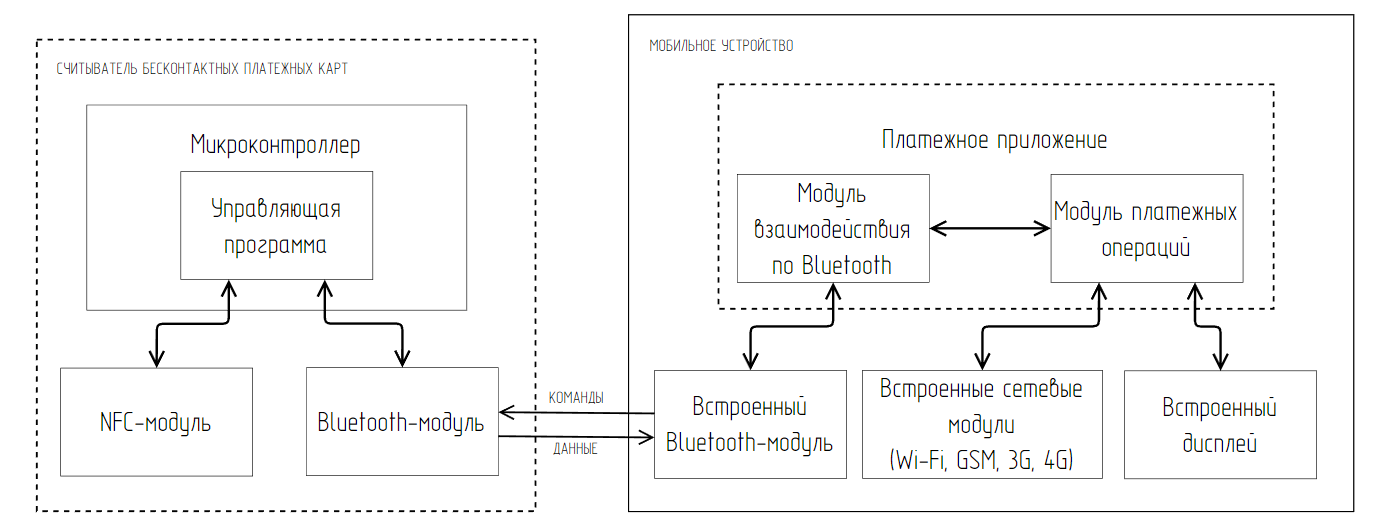
\includegraphics[width=0.8\textwidth]{images/design/struct_scheme}
    \caption{\centering Структурная схема системы}
    \label{fig:struct_scheme}
\end{figure}

Считыватель бесконтактных платежных карт включает в себя 3 аппаратных модуля в соответствии с требованиями ТЗ:
\begin{itemize}
    \item Bluetooth-модуль для связи с мобильным устройством, которое осуществляет выполнения платежных операций;
    \item NFC-модуль для взаимодействия с бесконтактной средством платежа;
    \item микроконтроллер для осуществления управления устройством (контроля работы NFC-модуля и Bluetooth-модуля).
\end{itemize}

Для микроконтроллера реализуется ПО, с помощью которого осуществляется управления NFC и Bluetooth модулями, через предоставляемые модулями интерфейсы для управления, описанных в их документации (форматом управляющих команд).
NFC-модуль подключается посредством разъема SPI, Bluetooth-модуль подключается посредством разъема USART для передачи управляющих команд с необходимыми данными.


Мобильное приложение включает в себя следующие программные модули:
\begin{itemize}
    \item модуль взаимодействия с устройством считывателем по Bluetooth,
    \item модуль платежных операций для сетевых запросов к API банка-эквайера.
\end{itemize}

Используются следующие аппаратные модули мобильного устройства:
\begin{itemize}
    \item Bluetooth-модуль для взаимодействия со считывателем,
    \item встроенные сетевые модули (Wi-Fi, GSM, 3G, 4G) для взаимодействия с сервером банка-эквайера,
    \item дисплей для взаимодействия с пользователем.
\end{itemize}

Структурная схема с внешними участниками процесса оплаты представлена на рисунке~\ref{fig:struct_scheme_out}.
На ней также указаны направления обмена данными между программными, аппаратными модулями и внешними участниками процесса оплаты.

\begin{figure}[H]
    \centering
    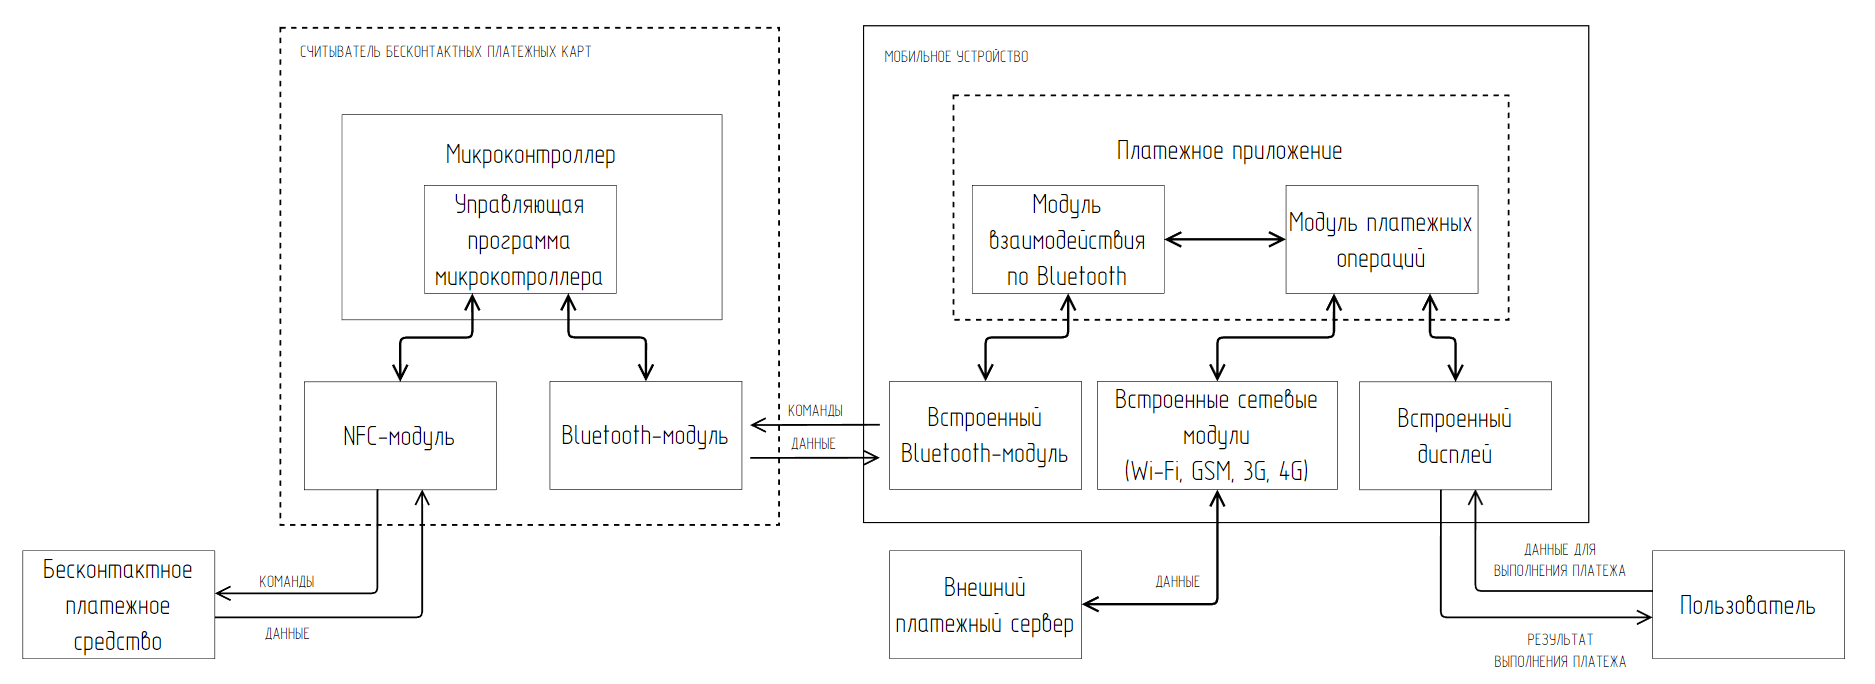
\includegraphics[width=1\textwidth]{images/design/struct_scheme_out}
    \caption{\centering Структурная схема системы с внешними участниками процесса оплаты}
    \label{fig:struct_scheme_out}
\end{figure}


\subsection{Разработка аппаратной части системы}

\subsubsection{Функциональная схема аппаратной части системы}

В соответствии с требованиями технического задания основные функции аппаратной части системы (микроконтроллерной системы):
\begin{itemize}
    \item взаимодействие со средством платежа посредством технологии NFC в соответствии со стандартом взаимодействия с бесконтактными средсвами платежа EMV Contactless, рассмотренном в исследовательской части;
    \item связь с мобильным устройством посредством технологии Bluetooth (получение управляющих команд и отправка полученных данных).
\end{itemize}

В данном процессе задействуется МК, Bluetooth-модуль и NFC-модуль.
Все эти компоненты работают как единая система под управлением МК.

% TODO нарисовать схему работы (диаграмму последовательностей)
Алгоритм работы устройства:
\begin{enumerate}
    \item настройка Bluetooth-модуля для подключения к мобильному устройству;
    \item установка соединения мобильного устройства и Bluetooth-модуля;
    \item получение команды от мобильного устройства о начале транзакции и суммы транзакции;
    \item включение и базовая настройка NFC-модуля микроконтроллером, начало поиска средства платежа;
    \item обнаружение средства платежа, установка соединения и взаимодействие с ним в соответствии алгоритмом представленном на рисунке~\ref{fig:kernel_transaction_flow}; % TODO: нарисовать mir_transaction и заменить
    \item передача полученных данных от средства платежа на мобильное устройство посредством Bluetooth;
\end{enumerate}

Структурная схема устройства представлена на рисунке~\ref{fig:apparat_struct}.
На ней NFC-модуль имеет детализированное изображение с целью демонстрации комплексности структуры данного устройства.

\begin{figure}[h]
    \centering
    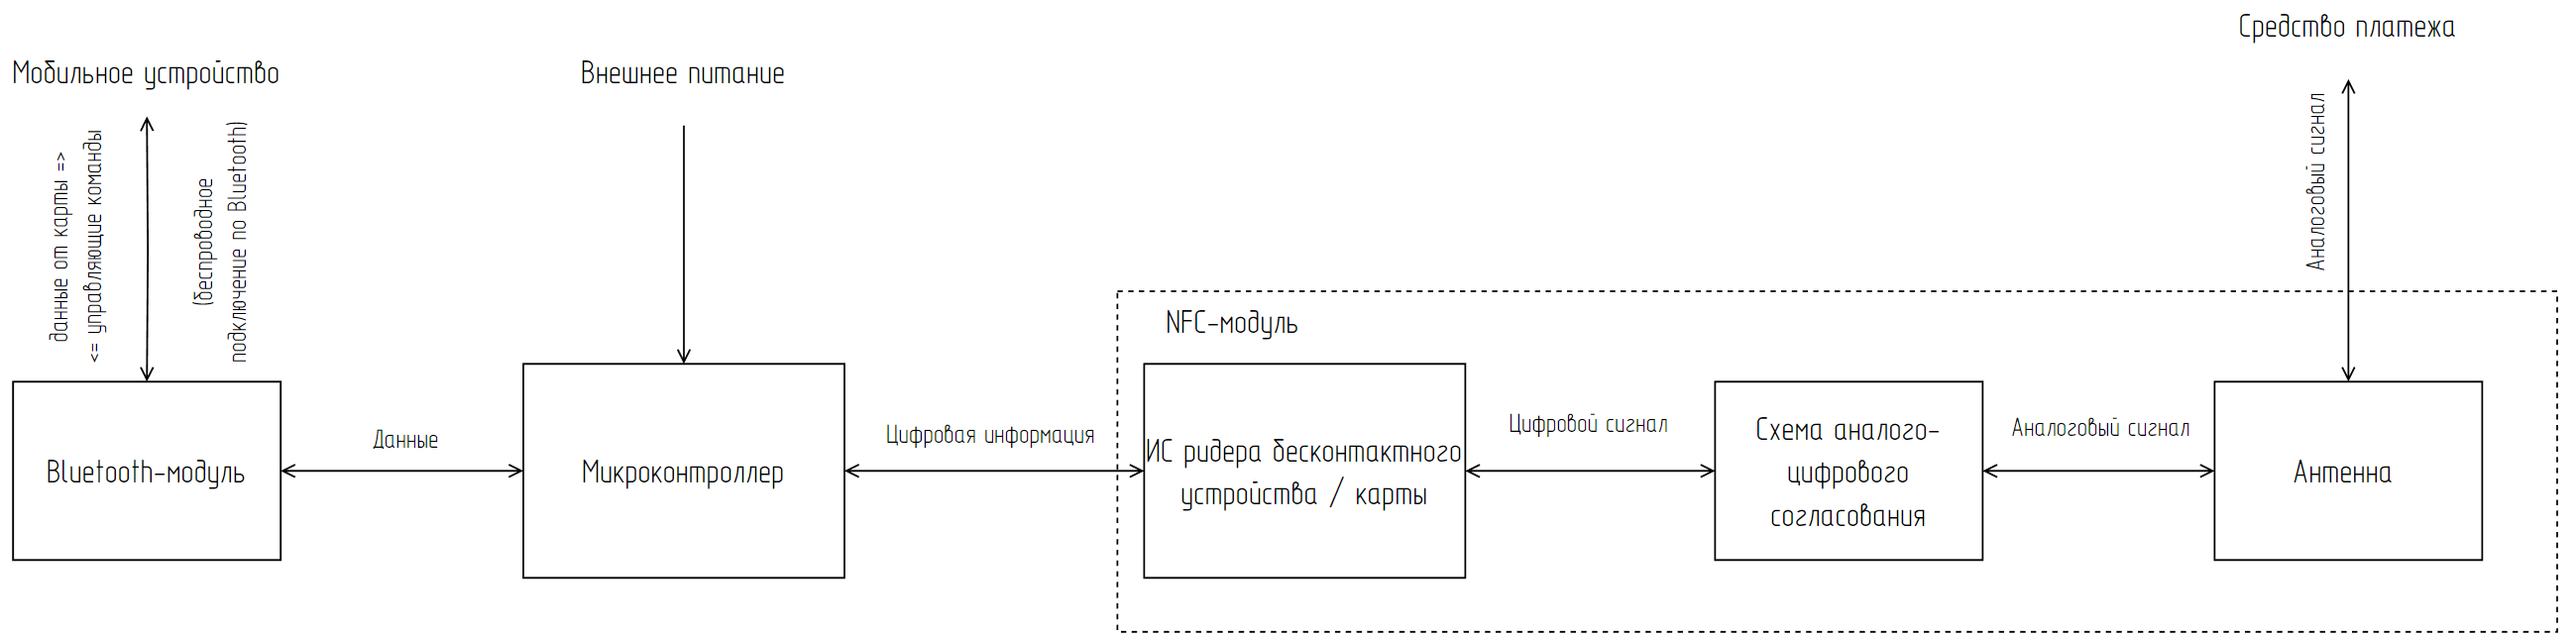
\includegraphics[width=1\textwidth]{images/design/apparat_struct}
    \caption{\centering Структурная схема считывателя бесконтактных платежных карт}
    \label{fig:apparat_struct}
\end{figure}


Согласно требованию ТЗ разрабатываемое устройство должно обеспечивать возможность подключения по Bluetooth к мобильному устройству, с возможностью приема и передачи данных, также оно должно взаимодействовать с бесконтактным средством платежа в соответствии со стандартом ISO/IEC 14443 с помощью модуля NFC, поддерживающему работу с картами ПС <<МИР>>.
Данные модули должны работать под управлением МК, имеющего разъемы SPI и USART для их подключения.
При этом стандарта EMV Contactless вводит строгие временные ограничения на время прямого непосредственного взаимодействия с картой (не более 0.4 мс).
Из чего следует, что МК должен обладать высокой производительностью.
ISO/IEC 14443-A используемый в платежных картах обладает скоростью передачи данных 106 кбит/с или 13.25 кбайт/с, что с учетом используемого компактного формата TLV для передаваемых сообщений и их размера, который значительно меньше чем объем, предаваемый даже за 1 мс, не создает ограничений по производительности.

При анализе существующих mPOS-терминалов было установлено, что они используют микропроцессоры с архитектурой Advanced RISC Machines (ARM), в частности ARM 7, ARM 9, ARM 11, которые обладают частотой более 100 МГц.
С учетом того, что данные терминалы используются для обработки транзакций различных платежных систем и не только бесконтактным образом для разрабатываемой системы данные процессоры будут избыточны, однако использование ARM архитектуры было бы крайне желательно.

В таблице~\ref{tab:microcontroller_comparison} приведены характеристики различных микроконтроллеров от разных компаний~\cite{stm32f103_datasheet}\cite{atmega328p_datasheet}.

\begin{longtable}[l]{|
P{0.18\textwidth}|
P{0.2\textwidth}|
P{0.15\textwidth}|
P{0.13\textwidth}|
P{0.2\textwidth}|}

    \caption{Сравнение характеристик часто используемых микроконтроллеров}
    \label{tab:microcontroller_comparison} \\
    \hline
    \textbf{Характеристика} &
    \textbf{ATmega328P} &
    \textbf{ESP8266} &
    \textbf{PIC16F8} &
    \textbf{STM32F103} \\
    \hline
    \endfirsthead

    \caption*{Продолжение таблицы~\ref{tab:microcontroller_comparison}} \\
    \hline
    \textbf{Характеристика} &
    \textbf{ATmega328P} &
    \textbf{ESP8266} &
    \textbf{PIC16F8} &
    \textbf{STM32F103} \\
    \hline
    \endhead

    \hline
    \endfoot

    \hline
    \endlastfoot

    Разрядность процессора &
    8 бит &
    32 бит &
    8 бит &
    32 бит \\
    \hline

    Тактовая частота &
    до 20 МГц &
    до 160 МГц &
    до 20 МГц &
    до 72 МГц \\
    \hline

    Флэш-память &
    32 КБ &
    4 МБ &
    14 КБ &
    64 КБ \\
    \hline

    SRAM &
    2 КБ &
    160 КБ &
    368 Б &
    20 КБ \\
    \hline

    EEPROM &
    1 КБ &
    Нет &
    256 Б &
    Нет \\
    \hline

    Количество I/O портов &
    23 &
    11 &
    13 &
    37 \\
    \hline

    Поддержка Wi-Fi &
    Нет &
    Да &
    Нет &
    Нет \\
    \hline

    Поддержка Bluetooth &
    Нет &
    Нет &
    Нет &
    Нет \\
    \hline

    Стоимость &
    Низкая &
    Низкая &
    Низкая &
    Низкая \\
    \hline
\end{longtable}

В ходе выполнения курсовой работы по дисциплине <<Микропроцессорные системы>> выбор был сделан в пользу микроконтроллера ATmega328P в составе платы Arduino Uno R3.
Данный вариант был удобен при первоначальном макетировании системы и изучении стандартов взаимодействия бесконтактной карты.
Однако частота данного МК значительно ниже чем у аналогов, у него 8-битная гарвардская архитектура процессора, при прочих равных Flash-памяти, SRAM, количество I/O-портов меньше чем у STM32F103.
Поэтому в качестве МК для аппаратной части системы используется STM32F103C8T6 на базе микропроцессора ARM Cortex-M3 с 32-битной архитектурой.
Данная архитектура позволяет работать с 32-битными регистрами, выполнять сложные математические операции, включая работу с плавающей запятой (с помощью программных или аппаратных средств).
Поддержка современных продвинутых программных библиотек, таких как HAL (Hardware Abstraction Layer), LL (Low Layer) и CMSIS (Cortex Microcontroller Software Interface Standard), предоставляет разработчику полный контроль над аппаратной частью микроконтроллера, с пониманием происходящих процессов на уровне регистров и таймеров.
В то же время, использование ATmega328P с Arduino.h для аналогичных задач часто приводит к неэффективному использованию ресурсов, ограничению функциональности и снижению производительности.
Кроме того, экосистема STM32 предоставляет мощные инструменты разработки, такие как STM32CubeIDE, которые упрощают настройку периферии и генерацию кода, сохраняя при этом гибкость и контроль над аппаратными ресурсами.

Для реализации беспроводного Bluetooth-соединения был выбран Bluetooth-модуль HC-05, обладающий следующими характеристиками:

\begin{itemize}
    \item напряжение питания: 3,3 В – 5 В;
    \item потребляемый ток: при подключении – до 40 мА (поиск, сопряжение, подключение), при передаче данных – до 8 мА;
    \item частотный диапазон: 2,4 ГГц – 2,48 ГГц;
    \item мощность передатчика: до +4 дБм;
    \item дальность связи: до 10 метров;
    \item интерфейс: USART;
    \item поддерживаемые скорости передачи данных: 9600, 19200, 38400, 57600, 115200, 230400 и 460800 бит/сек;
    \item режимы работы: Master (ведущий) и Slave (ведомый);
\end{itemize}

К преимуществам модуля HC-05 относятся дальность связи до 10 метров, поддержка скорости передачи данных до 460800 бит/сек и работа как в режиме Master (ведущий), так и в режиме Slave (ведомый).
Единственным недостатком является не самая актуальная версия технологии Bluetooth 2.0.
Однако даже модуль HC-08 имеет версию 4.0 (актуальная~-- 6.0) при стоимости в 4--5 раз выше и большим энергопотреблением.
Т.к. осуществляется процедура передачи данных без необходимости частого и многоразового подключения устройства-хоста к Bluetooth-модулю, а приоритетом является низкое энергопотребление – стандарт Bluetooth 2.0 является преимуществом, а не недостатком.

Модуль HC-05 можно настроить с помощью AT-команд, которые отправляются через интерфейс USART.
Это позволяет изменить имя устройства, пароль для подключения, скорость передачи данных и другие параметры.
Примеры AT-команд:

\begin{itemize}
    \item AT – проверка связи с модулем;
    \item AT+NAME=NewName – изменение имени модуля;
    \item AT+UART=9600 – установка скорости передачи данных на 9600 бод.
\end{itemize}

Модуль HC-05 включает в себя чип BC417143 и работает на напряжении 5 В и реализуя прием и передачу сигнала.


Среди прочих NFC-модулей наиболее популярными являются модули компании NXP.
К тому они имеют качественную и исчерпывающую документацию.
NXP поставляет не только NFC-модули, но и микроконтроллеры с интегрированными модулями NFC, а также разрабатывает ПО для работы с модулями, однако только для МК собственного производства.

В качестве модуля для считывателя используется NXP PN5180.
Данный модуль имеет поддержку большого числа стандартов технологии NFC.
Имеет сравнительно низкую стоимость (порядка 700--1000 рублей на ноябрь 2024 года).
А также имеет широкий функционал и подробную документацию.
PN5180 является широко распространенным модулем, с поддержкой множества стандартов (в том числе и используемого в платежах~-- ISO14443-A).
Альтернативой ему могут выступать схожие модули от компании NXP, в частности PN5190 (улучшенная версия PN5180), однако он умеет выше стоимость и при этом улучшения в производительности и поддержки стандартов пренебрежимо малы в рамках данного устройства.

%Основные внутренние компоненты интегральной схемы модуля представлены на рисунке~\ref{fig:pn5180_components}~\cite{pn5180_datasheet}.
%
%\begin{figure}[H]
%    \centering
%    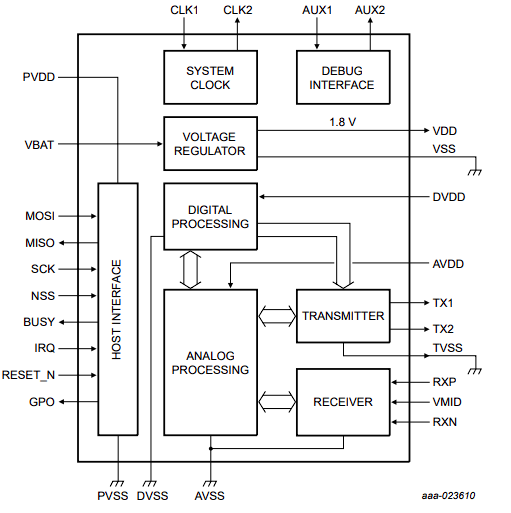
\includegraphics[width=0.8\textwidth]{images/design/pn5180_components}
%    \caption{\centering Компоненты интегральной схемы модуля PN5180}
%    \label{fig:pn5180_components}
%\end{figure}

Важно отметить, что производитель модуля предварительно выполняет следующие действия по его настройке:
\begin{itemize}
    \item определение целевого импеданса для оптимизации мощности RF-выхода и минимизации потребление энергии;
    \item проектирование EMC-фильтра для подавления нежелательных гармоник тока, которые могут создавать помехи в работе устройств;
    \item измерение LCR-параметров антенны (индуктивности, емкости и сопротивления) для работы;
    \item расчет компонентов для согласования антенны с NFC-модулем.
\end{itemize}

Также производится симуляция работы антенны, тестирование работы в реальных условиях и корректировка РЧ контура.
В результате чего получается надежный и стабильно работающий модуль, для которого нет необходимости в выполнении данных затруднительных действий, требующих дополнительного оборудования и навыков.


PN5180 использует для связи с микроконтроллером SPI, расширенный линией BUSY, что позволяет ему указыать о невозможности приема и отправки данных в конкретный момент времени.
Максимальная скорость его разъема SPI составляет 7 Мбит/с, при этом параметры SPI устанавливаются следующим образом: CPOL=0, CPHA=0 (SPI Mode 0), старший бит первым (MSB first).
На модуль по SPI передаются управляющие команды, список которых приведен в его datasheet в разделе <<Работа модуля NFC>>, с помощью этих команд происходит настройка модуля\cite{pn5180_datasheet}.

Уровень напряжения сигналов, которыми оперирует модуль, составляет 1,8--3,3 В.
У STM32F103C8T6 рабочий уровень напряжения на разъемах~--- 3,3 В, что делает его совместимым с данным модулем.
В свою очередь на разъемах микроконтроллера ATmega328P рабочим уровнем напряжения является 5 В, что усложняло его использование в первом разработанном макете устройства (возникала необходимость использования конвертера уровня напряжения, что повышало количество энергии, потребляемое МК-системой).


На функциональной схеме изображены используемые компоненты, необходимые для работы устройства, также показаны подключения модулей и используемые для этого контакты, направления передачи данных и управляющих сигналов.
Спроектированная функциональная схема разработанного устройства представлена в приложении~В.
На схеме МК изображены только используемые компоненты.




\subsubsection{Принципиальная схема аппаратной части системы}

%\paragraph{Программирование МК}

Программирование микроконтроллера STM32F103C8T6 осуществляется с использованием интерфейса SWD (Serial Wire Debug), который является стандартным решением для отладки и прошивки большинства 32-битных ARM-микроконтроллеров.
Интерфейс SWD разработан для упрощенного подключения к микроконтроллеру, в отличие от JTAG, он использует минимальное количество выводов, что делает его особенно удобным в условиях ограниченного пространства на плате.

Для работы с этим интерфейсом необходимы всего два сигнальных контакта:
\begin{itemize}
    \item SWCLK — тактовая линия;
    \item SWDIO — двунаправленная линия передачи данных.
\end{itemize}

Также требуются линии питания и земли:
\begin{itemize}
    \item VCC — питание 3.3 В;
    \item GND — общий провод.
\end{itemize}

Процесс программирования выглядит следующим образом:

\begin{enumerate}
    \item программатор ST-Link v2 подключается к микроконтроллеру через разъем, соответствующий интерфейсу SWD;
    \item программатор устанавливает связь с ядром микроконтроллера, отправляя тактовые сигналы по линии SWCLK и управляя данными через SWDIO;
    \item происходит загрузка и запись кода во флэш-память микроконтроллера;
    \item МК автоматически перезапускается для исполнения загруженную программы.
\end{enumerate}

Таким образом, для программирования микроконтроллера STM32F103C8T6 через ST-Link v2 используется разъем SWD, представленный на рисунке~\ref{fig:swd}.

\begin{figure}[H]
    \centering
    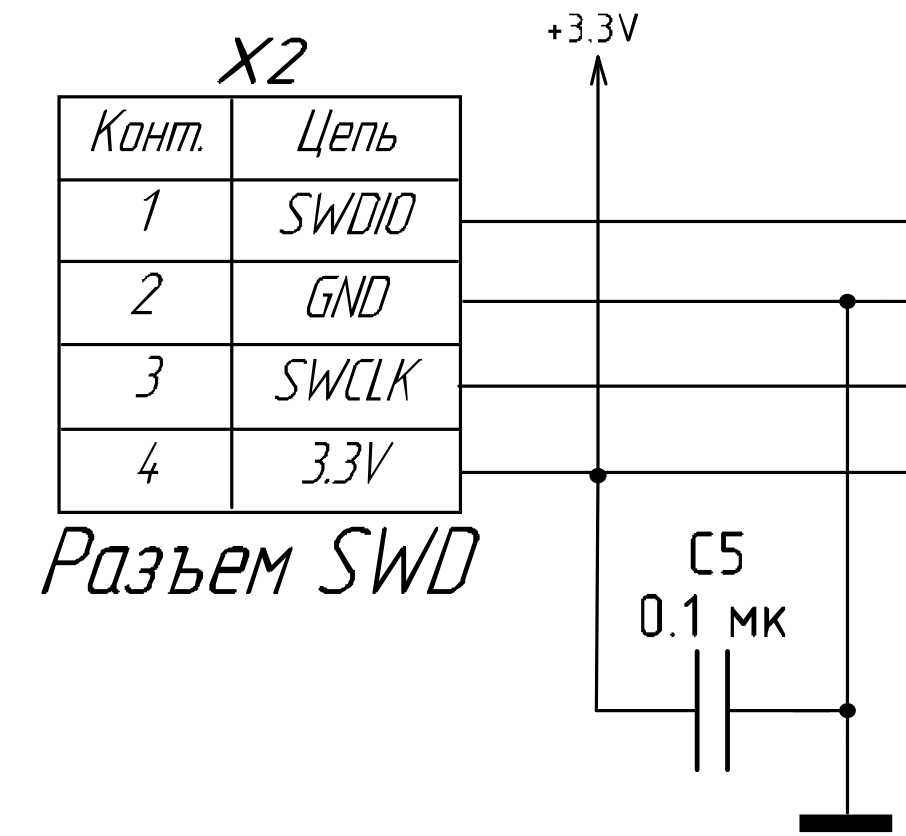
\includegraphics[width=0.3\textwidth]{images/design/swd}
    \caption{\centering Разъем программирования МК}
    \label{fig:swd}
\end{figure}

%\paragraph{Подключение цепи питания}

Для обеспечения работоспособности устройства необходимо подавать стабилизированное напряжение на микроконтроллер и прочие компоненты схемы.
В данной МК-систем питание микроконтроллера STM32F103C8T6 осуществляется через стандартный USB-разъём microUSB, который используется как интерфейс подключения к внешнему источнику питания.
Это позволяет отказаться от использования дополнительного внешнего источника питания и упрощает конструкцию устройства.
Разъем представлен на рисунке~\ref{fig:usb}.

\begin{figure}[H]
    \centering
    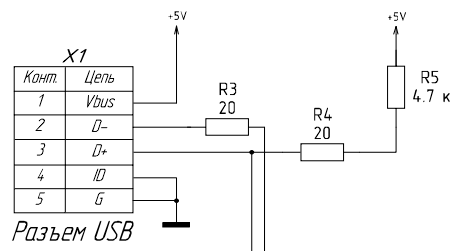
\includegraphics[width=0.4\textwidth]{images/design/usb}
    \caption{\centering Разъем питания МК}
    \label{fig:usb}
\end{figure}

Напряжение с USB поступает непосредственно на стабилизатор напряжения RT9193--33, т.к. микроконтроллер STM32F103C8T6 работает на напряжении 3.3 В, а не 5 В, как это часто бывает в других МК.
Стабилизатор преобразует напряжение с USB (5 В) к необходимому уровню и обеспечивает стабильное питание ядра и периферийных модулей микросхемы.

Для фильтрации питающего напряжения используются керамических конденсаторы, установленные на входе и выходе стабилизатора.
Такое решение обеспечивает минимальный уровень шума и стабильную работу микроконтроллера.
Емкости конденсаторов определены в соответствии с документацией STM32F103C8T6~\cite{stm32f103_datasheet}.

Схема стабилизации и понижения напряжения представлена на рисунке~\ref{fig:mk_usb_stab}.

\begin{figure}[H]
    \centering
    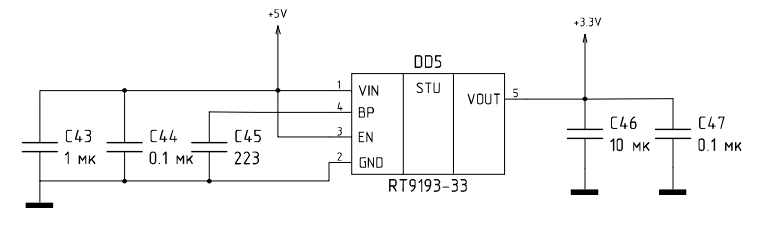
\includegraphics[width=0.6\textwidth]{images/design/mk_usb_stab}
    \caption{\centering Схема стабилизации питания МК-системы}
    \label{fig:mk_usb_stab}
\end{figure}

%\paragraph{Расчет сопротивления резисторов}

На принципиальной схеме расположено несколько резисторов.

Резистор R1 используется для стабилизации тока на источнике тактирования.
Резистор R2 используется для подтягивания линии RESET до 3.3~В.
Их номиналы установлены согласно документации на микроконтроллер\cite{stm32f103_datasheet}.

Резисторы R2--R5 добавлены для токоорганичния разъема USB, который используется для питания.

В Bluetooth-модуле, согласно документации, Резисторы R6, R9 имеют номинал 220~кОм и 1~кОм соответственно, а R7, R8~--- 10~кОм.

В состав NFC-модуля PN5180, согласно документации, входят резисторы R10, R13 сопротивлением 4.7 кОм и R11, R12, R14, R15 сопротивлением 2.2~кОм.

Дополнительно хотелось бы отметить, что расчет сопротивлений, емкостей и индуктивностей для PN5180 производился на основе раздела datasheet <<17.1 Typical component values>>\cite{pn5180_datasheet}.
В нем приведена схема с минимальным количеством компонентов и значения для них, представленные на рисунках~\ref{fig:pn5180mincomp} и~\ref{fig:pn5180mincompvalues} соответственно.

\begin{figure}[H]
    \centering
    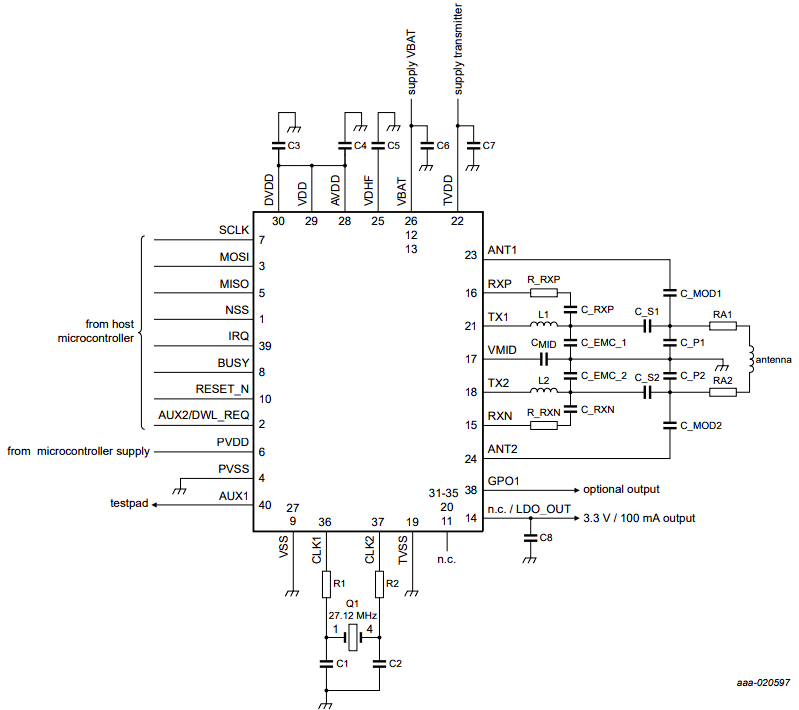
\includegraphics[width=0.7\textwidth]{images/design/pn5180mincomp}
    \caption{\centering Схема модуля PN5180 с минимальным набором элементов}
    \label{fig:pn5180mincomp}
\end{figure}

\begin{figure}[H]
    \centering
    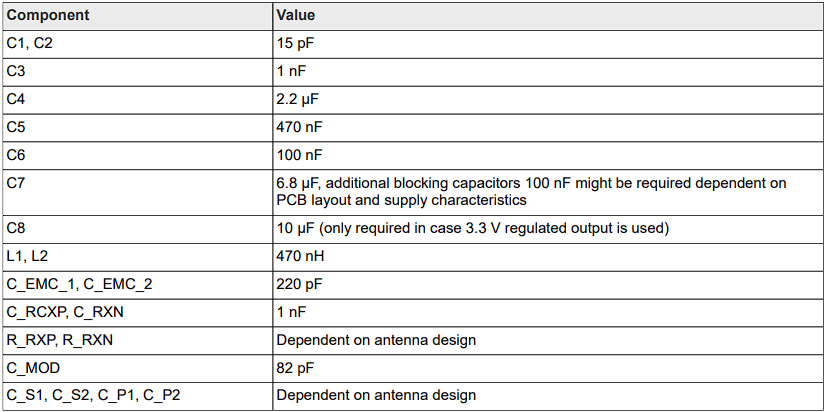
\includegraphics[width=0.7\textwidth]{images/design/pn5180mincompvalues}
    \caption{\centering Значения для элементов PN5180}
    \label{fig:pn5180mincompvalues}
\end{figure}

Также в открытом доступе находится принципиальная электрическая схема первой ревизии модуля PN5180 от производителя, которая и послужила основой для собственной электрической принципиальной схемы\cite{pn5180_schematic}.

% TODO: Подключение модулей

На основе всех вышеописанных сведений была спроектирована принципиальная схема разрабатываемой системы, показанная в приложении~Г.





\subsubsection{Макет аппаратной части системы}

В качестве МК для макета используется STM32F103C8T6 в составе отладочной платы Blue Pill, представленной на рисунке~\ref{fig:blue_pill}.

\begin{figure}[H]
    \centering
    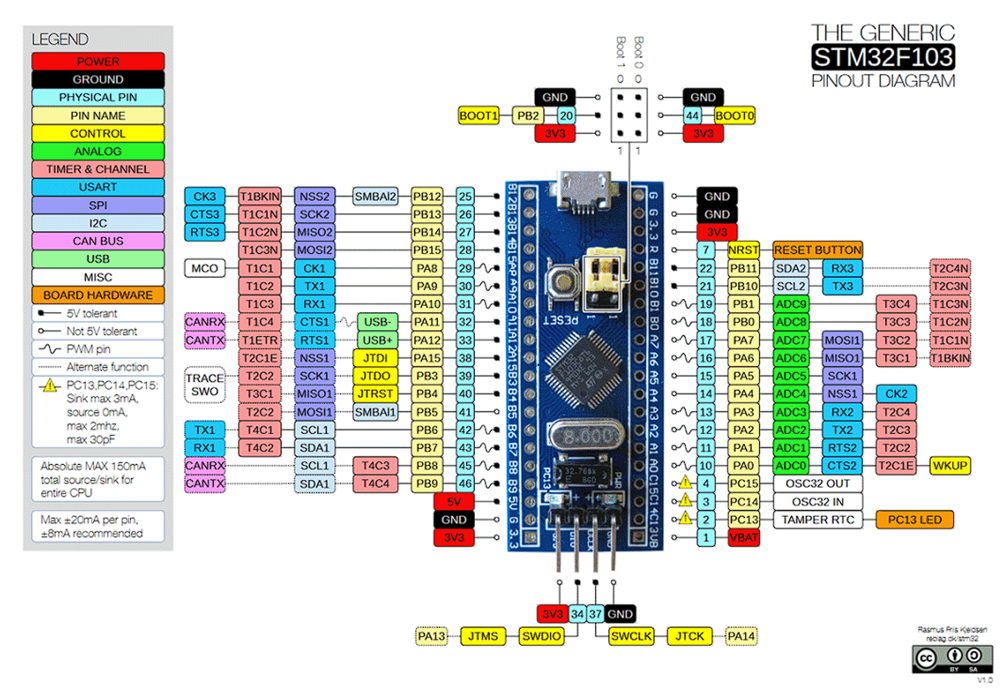
\includegraphics[width=0.8\textwidth]{images/design/blue_pill}
    \caption{\centering Отладочная плата Blue Pill с МК STM32F103C8T6}
    \label{fig:blue_pill}
\end{figure}

Сборка макета происходила в соответствии с принципиальной схемой из приложения~Г.
Макет представлен на рисунке~\ref{fig:maket}.

\begin{figure}[H]
    \centering
    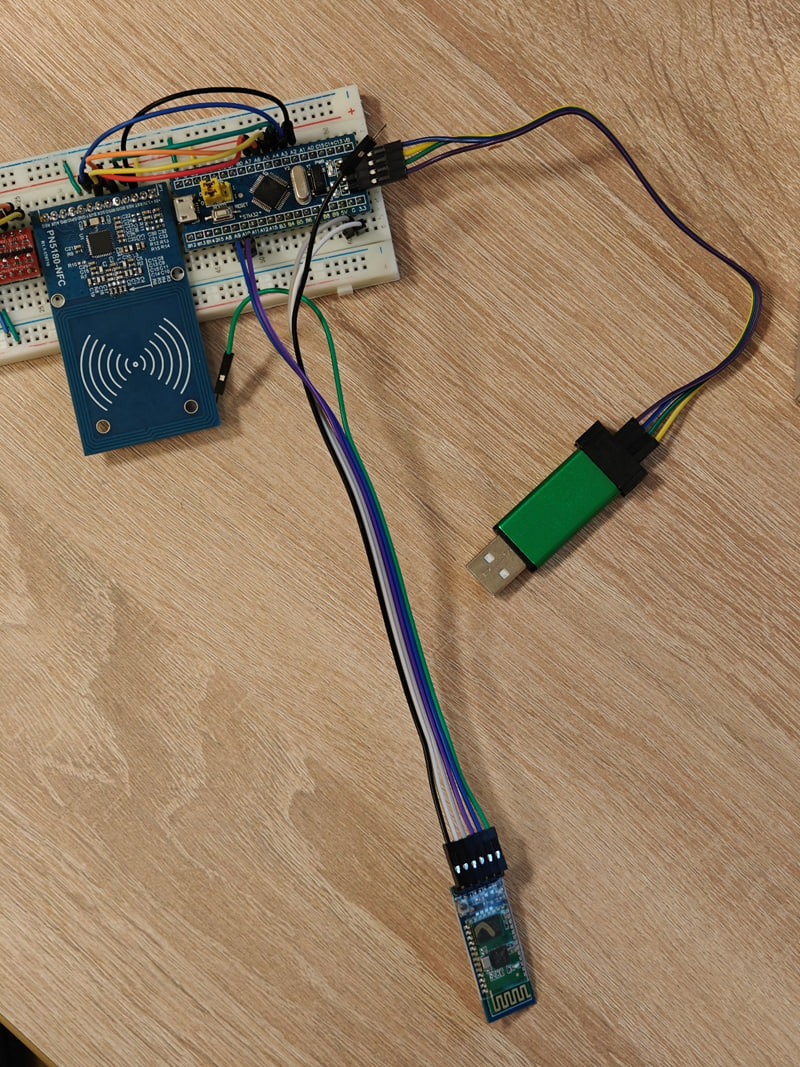
\includegraphics[width=0.5\textwidth]{images/design/maket}
    \caption{\centering Собранный макет устройства}
    \label{fig:maket}
\end{figure}

Для разработанного устройства-считывателя также был произведен расчет мощности.
Мощность, потребляемая разработанной схемой, складывается из мощностей, потребляемых всеми устройствами из ее состава.
Из документации используемых устройств получена информация, приведенная в таблице~\ref{tab:power}.
Расчет максимальной мощности, потребляемой устройством, определяется по формуле:

$$
P_{max} = \sum_{i=1}^{k} U_i \cdot I_{i_{max}} \cdot n_i,
$$
где $U_i$~--- напряжение питания устройства, $I_{i_{max}}$~--- максимальный ток потребления, $n_i$~--- количество элементов в системе.

\begin{longtable}[l]{|
P{0.23\textwidth}|
P{0.15\textwidth}|
P{0.15\textwidth}|
P{0.15\textwidth}|
P{0.2\textwidth}|}

    \caption{Сравнение микросхем по потребляемой мощности}
    \label{tab:power} \\
    \hline
    \textbf{Микросхема} &
    \textbf{Ток потребления, мА} &
    \textbf{Потребляемая мощность, мВт} &
    \textbf{Количество устройств} &
    \textbf{Суммарная мощность, мВт} \\
    \hline
    \endfirsthead

    \caption*{Продолжение таблицы~\ref{tab:power}} \\
    \hline
    \textbf{Микросхема} &
    \textbf{Ток потребления, мА} &
    \textbf{Потребляемая мощность, мВт} &
    \textbf{Количество устройств} &
    \textbf{Суммарная мощность, мВт} \\
    \hline
    \endhead

    \hline
    \endfoot

    \hline
    \endlastfoot

    STM32F103\-C8T6 & 10 & 50 & 1 & 50 \\ \hline

    BC417143 & 70 & 231 & 1 & 231 \\ \hline

    PN5180A0NH & 20 & 60,6 & 1 & 60,6 \\ \hline

    R1114-3.3 & 100 & 500 & 1 & 500 \\ \hline

    CD1206-S01575 & 150 & 750 & 1 & 750 \\ \hline

    LP2985-33DBVR & 150 & 750 & 1 & 750 \\ \hline

    NCP1117-ST50T3G & 800 & 4500 & 1 & 4500 \\ \hline
\end{longtable}

При питании 5 В суммарная мощность системы будет приблизительно равна 6,342 Вт.

% TODO: make correct расчет потребляемой мощности


\subsection{Разработка программной части системы}

\subsubsection{Программа считывателя платежных средств}

% todo: добавить рисунок для mir

В основу алгоритмов работы устройства легли алгоритмы, представлены на рисунках~\ref{fig:pcd_flow} и~\ref{fig:pcd_flow_2_picc_activation},~\ref{fig:transaction_flow_example} и~\ref{fig:kernel_transaction_flow}, а также алгоритмы из спецификации для ПС <<МИР>>~\cite{book_mir}.
На основе них были разработаны несколько алгоритмов:

\begin{itemize}
    \item выполнения платежной транзакции~--- рисунок~\ref{fig:complete_transaction};
    \item активации протокола ISO/IEC 14443--3~--- рисунок~\ref{fig:activate_iso3};
    \item активации протокола ISO/IEC 14443--4~--- рисунок~\ref{fig:activate_iso4};
    \item поиска платежных данных AFL~--- рисунок~\ref{fig:find_afl}.
\end{itemize}


\begin{figure}[H]
    \centering
    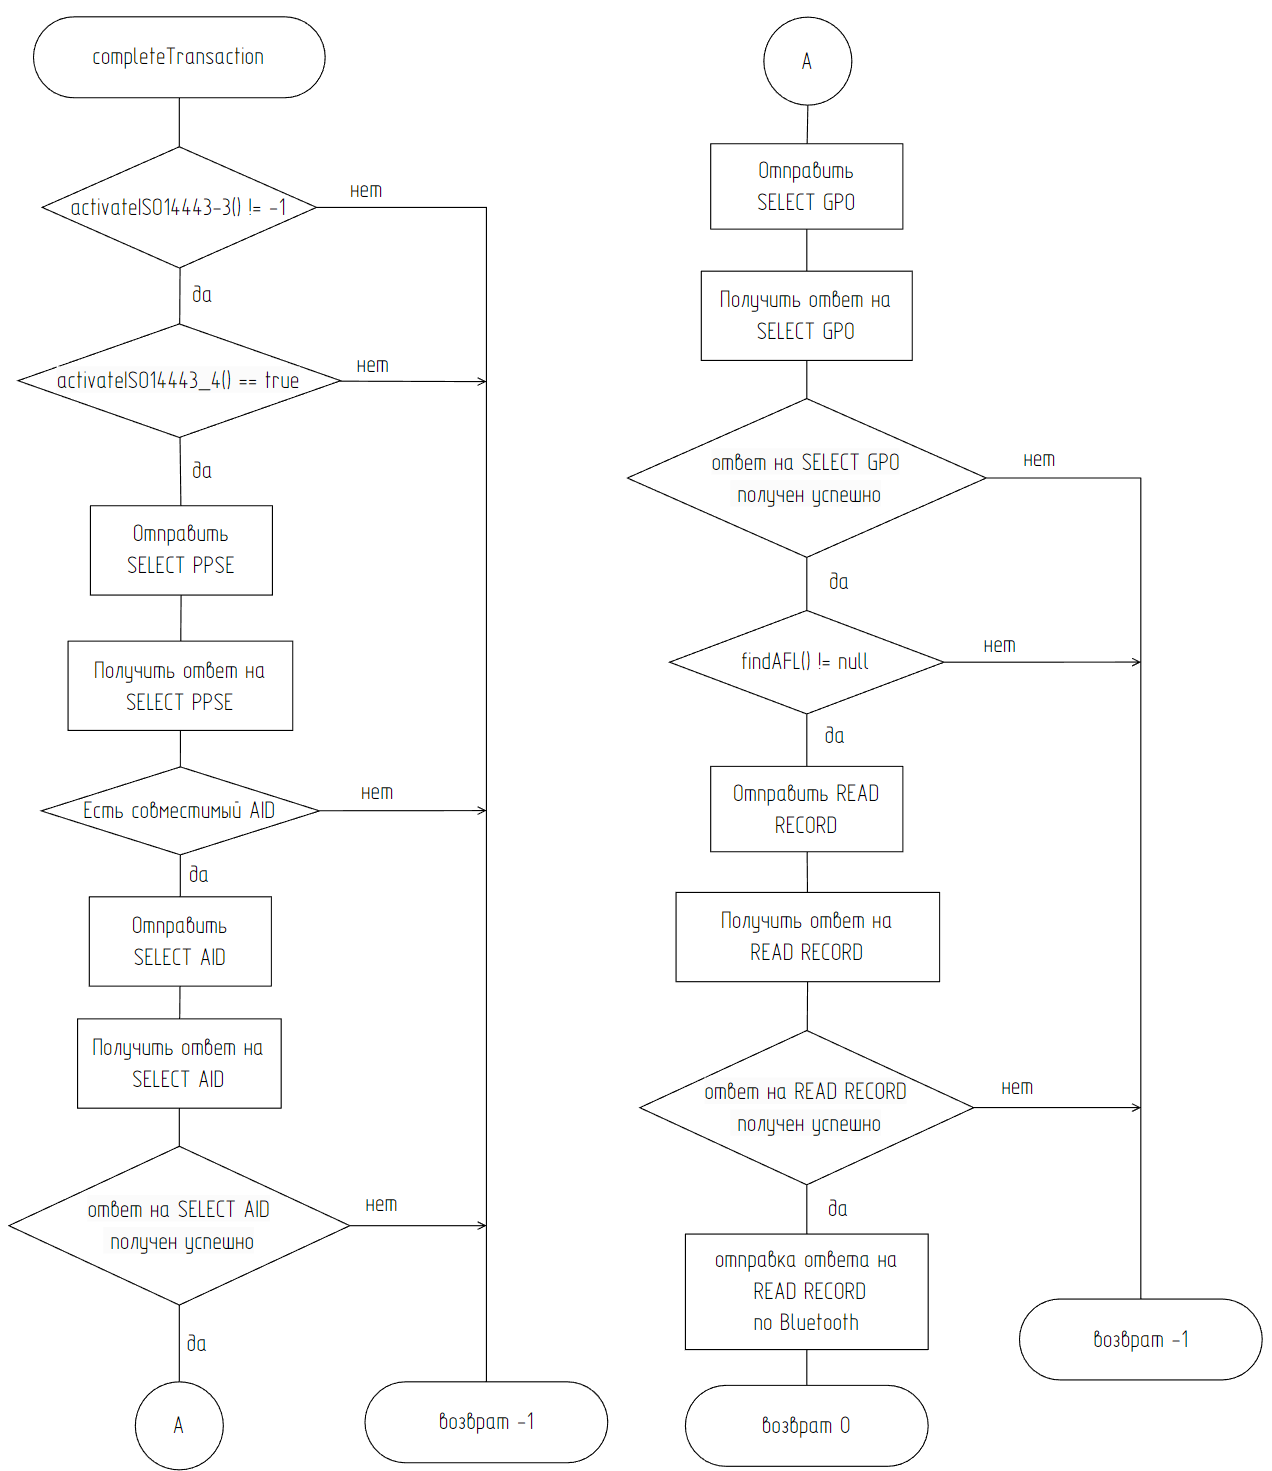
\includegraphics[width=0.8\textwidth]{images/design/complete_transaction}
    \caption{\centering Схема алгоритма выполнения платежной транзакции}
    \label{fig:complete_transaction}
\end{figure}

\begin{figure}[H]
    \centering
    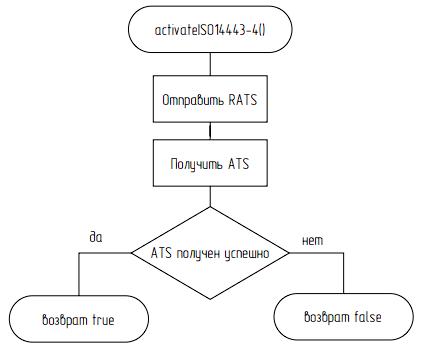
\includegraphics[width=0.5\textwidth]{images/design/activate_iso4}
    \caption{\centering Схема алгоритма активации протокола ISO/IEC 14443--4}
    \label{fig:activate_iso4}
\end{figure}

\begin{figure}[H]
    \centering
    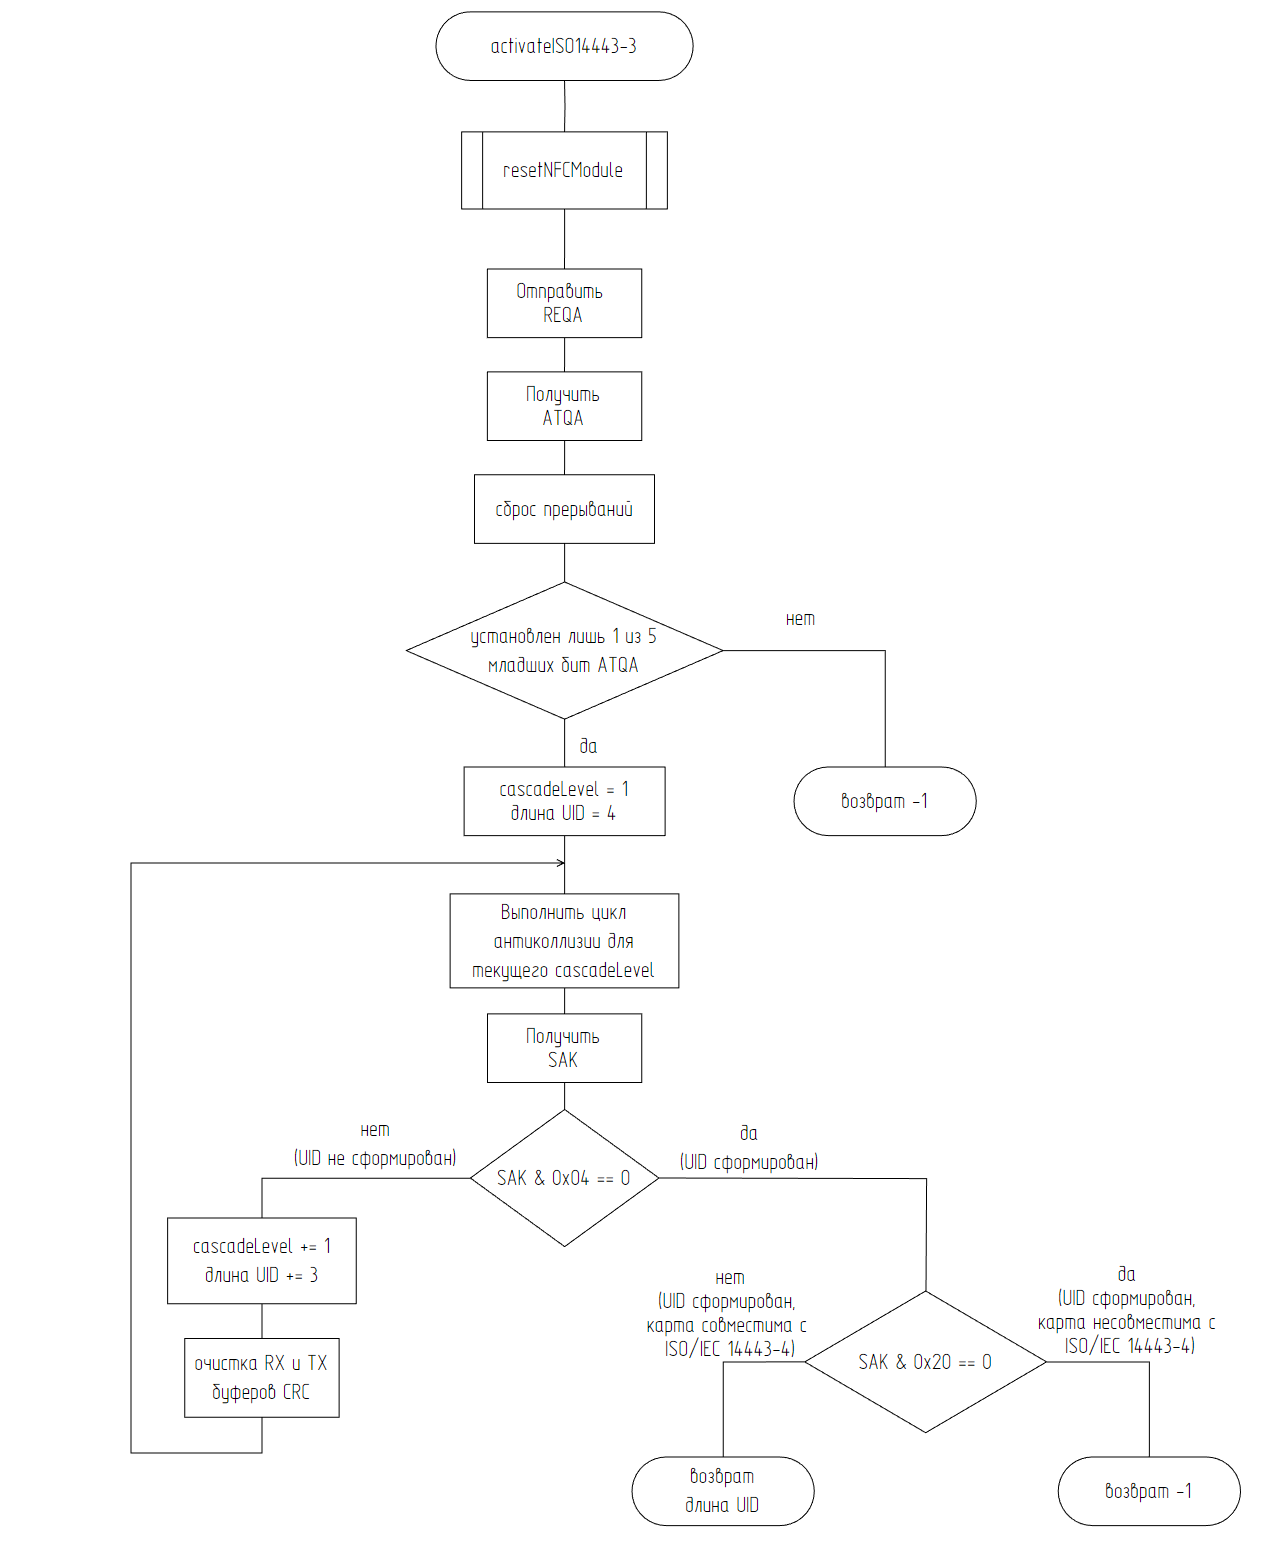
\includegraphics[width=0.9\textwidth]{images/design/activate_iso3}
    \caption{\centering Схема алгоритма активации протокола ISO/IEC 14443--3}
    \label{fig:activate_iso3}
\end{figure}

\begin{figure}[H]
    \centering
    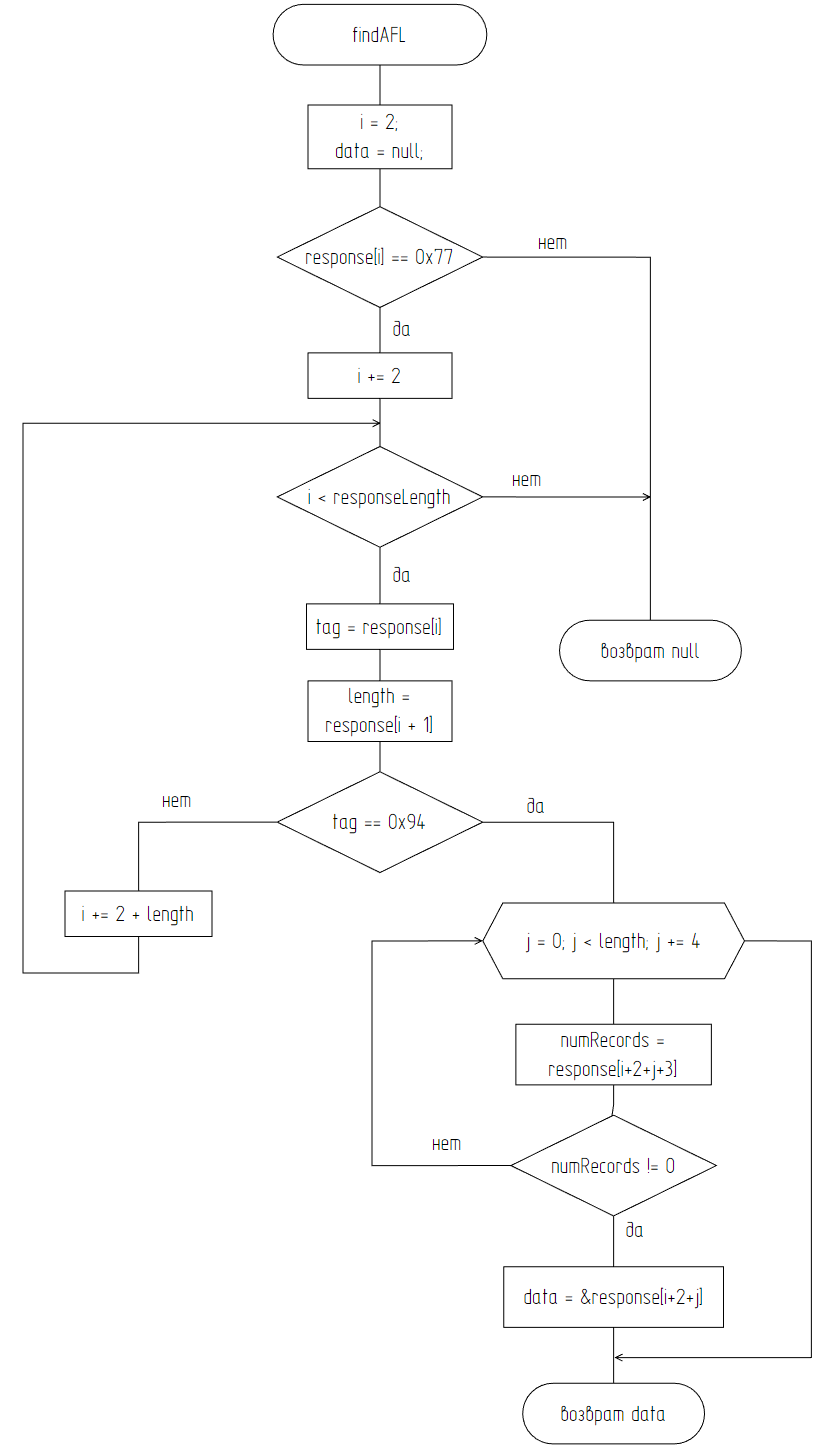
\includegraphics[width=0.7\textwidth]{images/design/find_afl}
    \caption{\centering Схема алгоритма поиска платежных данных AFL}
    \label{fig:find_afl}
\end{figure}


На рисунке~\ref{fig:find_afl} представлен алгоритм поиска значения тега Application File Locator (AFL), чтение которого является обязательным для формирования транзакции.
На основе найденного значения AFL формируется запрос чтения записи с карты~--- Read Record с указанием адреса, полученного в AFL.
Правила формирования следующие:

\begin{itemize}
    \item CLA = 0x00  - класс команды,
    \item INS = 0xB2 - тип инструкции (Read Record),
    \item P1 = Start - индекс первого байта,
    \item P2 = SFI|4 - второй параметр команды на основе SFI,
    \item Lc = 0x00 - ожидаемое количество байт в ответе (0 - любое).
\end{itemize}

Разработка программного обеспечения устройства происходила в среде STM32CubeIDE, предназначенной для разработки на микроконтроллерах серии STM32.
STM32 умеет производить компиляцию с файлов C и C++ с помощью gcc и g++.
В качестве основного языка программирования использовался C++, т.к. в отличие от C он предоставляет поддержку парадигмы объектно-ориентированного программирования.
Сама программа имеет модульный характер, на основе того, что в соответствие каждому аппаратному модулю (кроме МК) поставлен программный модуль, реализующий основные свойства и методы класса.

Настройка STM32F103C8T6 производилась с помощью графических средств STM32CubeIDE.
Пример такой настройки является настройка источника тактирования, представленная на рисунке~\ref{fig:stm_cube}.

\begin{figure}[H]
    \centering
    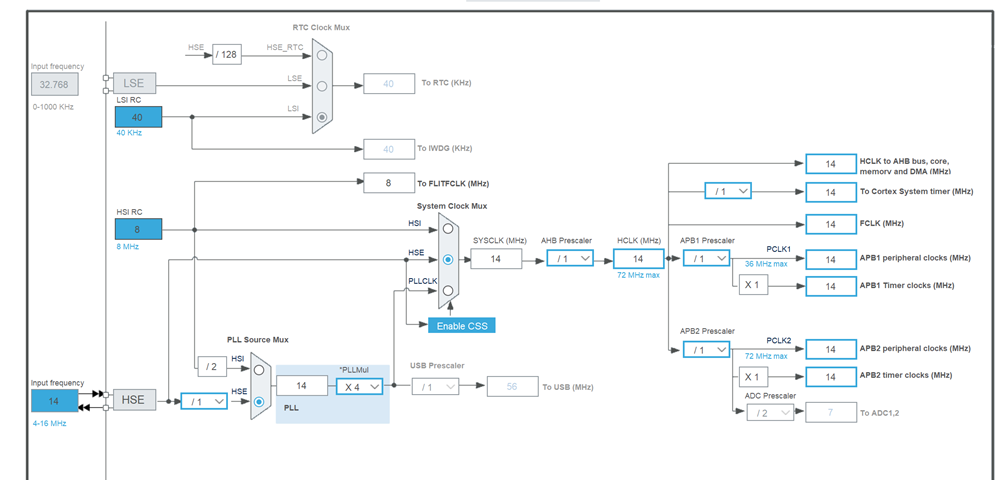
\includegraphics[width=1\textwidth]{images/design/stm_cube}
    \caption{\centering Настройка источника тактирования STM32F103C8T6}
    \label{fig:stm_cube}
\end{figure}

В качестве частоты используется 14 МГц для достижения максимальной скорости передачи данных с PN5180, который поддерживает максимальную скорость в 7 Мбит/с.
С помощью предделителя частоты SPI, равного 2, частота APB2 (именно к ней подключен SPI1) понижается до 7 МГц и 7 Мбит/с соответственно.
В приложении~Б приведены листинги со следующими фрагментами кода:
\begin{itemize}
    \item настройка SPI для подключения PN51804
    \item настройка USART для подключения Bluetooth-модуля HC-05.
\end{itemize}

Взаимодействие с PN5180 разделено на два класса PN5180 и PN5180ISO14443.
Первый описывает реализацию основных методов управления состоянием модуля, а второй реализует специфичные для стандарта ISO14443 методы работы, с помощью которых осуществляется взаимодействие NFC-модуля и платежного средства.
Примеры реализующих их процедур приведены в приложении~Б.


\subsubsection{Программа мобильного устройства}

В соответствии с требованиями ТЗ программа должна работать под управлением устройств с ОС Android версии 9 и выше.
Разрабатываемое программное обеспечение для мобильного устройства должно обеспечивать выполнение всех требуемых функций взаимодействия между считывателем бесконтактных карт и сервером банка-эквайера.
Управляющая программа будет работать на мобильном устройстве под управлением ОС Android и предоставлять пользовательский интерфейс для отслеживания состояния транзакции, её инициализации и получения результата.

Основные функции, выполняемые программой:
\begin{itemize}
    \item инициация взаимодействия между платежным средством (банковской картой или мобильным кошельком) и терминалом;
    \item взаимодействие с внешним сервером через протоколы HTTPS и REST API, с соблюдением требований стандарта PCI DSS;
    \item управление состоянием транзакции на основе данных, полученных от сервера и терминала, в соответствии с правилами EMV Transaction Processing и форматом сообщений ISO 8583;
    \item корректное завершение платежной операции, включая отображение результатов пользователю и передачу статуса транзакции.
\end{itemize}

Для начала транзакции программа использует данные, полученные от платежного терминала и карты.
Конкретный перечень полей определяется спецификой взаимодействия с каждой из поддерживаемых платежных систем.
При этом данные должны быть корректно интерпретированы и переданы на сервер эквайера через безопасное соединение.

Программа возвращает статус выполнения платежной операции в формате JSON, совместимом с REST API.
При этом максимальное время ожидания ответа от аппаратной части системы установлено на уровне 30 секунд, от внешнего сервера~--- 10 секунд.


Для реализации мобильного приложения была выбрана платформа Android SDK, так как она:
\begin{itemize}
    \item предоставляет полный доступ к низкоуровневым модулям, таким как Bluetooth и NFC;
    \item поддерживает современные протоколы шифрования и интеграции с REST API;
    \item обеспечивает гибкость в версионировании и обновлениях;
    \item использует Kotlin или Java, что позволяет писать чистый и понятный код, сохраняя высокую степень переносимости и производительности.
\end{itemize}

Для реализации сетевого взаимодействия используется Retrofit 2 и OkHttp, что обеспечивает:

\begin{itemize}
    \item удобную работу с REST API;
    \item поддержку TLS 1.2+;
    \item возможность добавления сложных заголовков, таких как авторизация и проверка целостности запросов.
\end{itemize}

Для тестирования и отладки применяются:

\begin{itemize}
    \item OkHttp Profiler — для контроля сетевых запросов;
    \item Mockk / JUnit — для автоматизированного тестирования бизнес-логики без необходимости использования реального терминала.
\end{itemize}

% TODO: диаграммы деятельности и чего-либо еще

На основе процесса выполнения транзакции, описанного в спецификации EMV и определенности действий, выполняемых устройством-считывателем, были определены основные сценарии использования приложения, также был сформирован список необходимых экранов:
\begin{itemize}
    \item авторизация,
    \item выбор устройства,
    \item создание платежа,
    \item ожидание инициализации карты,
    \item успех/ошибка при инициализации карты,
    \item ввод PIN-кода,
    \item ввод подписи,
    \item успех/ошибка при выполнении платежа.
\end{itemize}

Формы всех экранов представлены на рисунке~\ref{fig:screens}.

\begin{figure}[H]
    \centering
    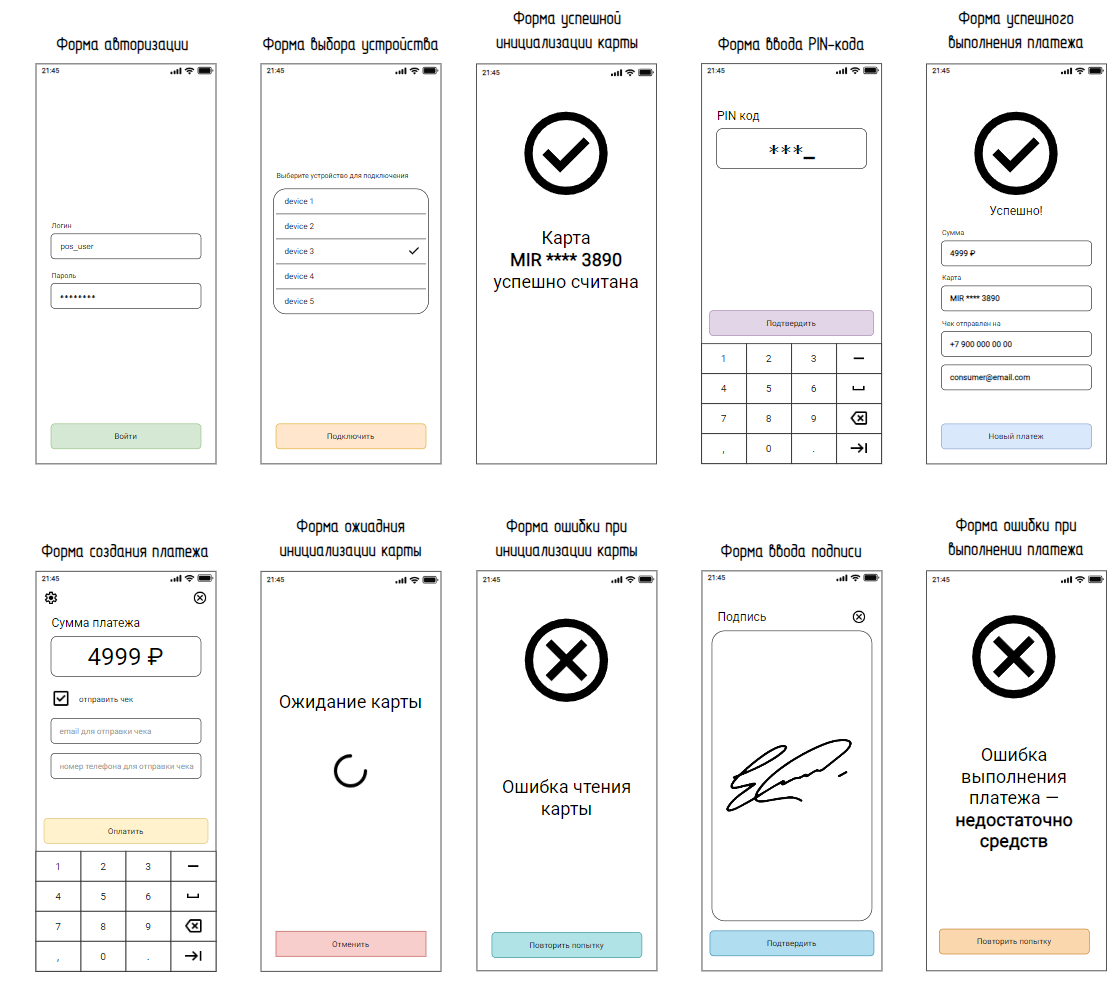
\includegraphics[width=0.9\textwidth]{images/design/screens}
    \caption{\centering Формы интерфейсы экранов}
    \label{fig:screens}
\end{figure}

Экран авторизации должен иметь поля для ввода логина и пароля, и выполнять аутентификацию и авторизацию пользователя приложения с помощью введенных логина и пароля по нажатию кнопки <<Войти>>.
В случае успешной авторизации выполняется переход на экран выбора устройства для подключения.
В случае ошибки отображается сообщение об ошибке в нижней части экрана, поля ввода логина и пароля очищаются, пользователь может повторно ввести их и повторить попытку авторизации.

На экране выбора устройства отображаются все доступные для подключения Bluetooth-устройства.
При первом открытие экрана выполняется проверка наличия разрешений на подключение и обнаружение устройств поблизости посредством Bluetooth.
По нажатию на устройство должно выполняться сопряжение и/или подключение к выбранному устройству.
Если выбранное устройство~--- считыватель бесконтактных карт, то он сигнализирует (передает данные) об этом после подключения.
В случае успешного подключения к считывателю выполняется переход на экран создания платежа.
В случае неудачного подключения отображается сообщение об ошибке в нижней части экрана, пользователь может повторить попытку подключения к считывателю.

На экране создания платежа пользователь находится только при наличии активного подключения к считывателю.
Он может ввести сумму оплаты, а также, при необходимости, номер телефона и/или электронную почту для отправки электронного чека об операции.
По нажатию на кнопку <<Настройка>> происходит переход к экрану выбору устройств.
По нажатию на кнопку <<Очистить>> происходит очистка полей ввода суммы транзакции, полей ввода номера телефона и/или электронной почты.
По нажатию на кнопку <<Оплатить>> валидируются введеные пользователем данные, в случае их корректности отображается экран ожидания инициализации карты, в случае некорректности некорректные поля подсвечиваются, ошибка выводится на экран.

При переходе на экран ожидания инициализации карты на считыватель передается команда о необходимости запуска NFC-модуля, после его активации выполняется поиск бесконтактного платежного средства и взаимодействие с ним по спецификации ПС.
Если данные процессы выполнены успешно, то приложение получает от считывателя все необходимые данные для формирования платежной транзакции и отображает экран успешной инициализации карты, в противном случае~-- экран ошибки инициализации карты, на котором есть кнопка <<Повторить попытку>>, запускающая повторную инициализацию NFC-модуля и взаимодействие с картой.

Карта посредством считывателя может запросить дополнительную проверку в виде ввода PIN-кода держателем карты, в этом случае открывается экран ввода PIN-кода, на котором держатель карты может ввести кода от своей платежной карты.
Также проверка может запросить в виде ввода подписи держателя карты.
И PIN-код, и подпись отправляются в запросе в банк-эквайер посредством REST API с целью аутентификации держателя карты, банк отвечает статусом проверки держателя карты.

После успешной инициализации и прохождении проверок (либо их отсутствия) отправляется запрос в банк-эквайер посредством REST API с суммой операции и всеми необходимыми данными для выполнения платежа.
Банк-эквайер возвращает данные о результате выполнения платежной транзакции.
В зависимости от результата либо отображается экран успешного выполнения транзакции с информацией о транзакции, либо отображается экран с описанием произошедшей ошибки.
Оба экрана позволяют по нажатию кнопки перейти на экран создания платежа и создать новую платежную транзакцию.


На основе данного описания экранов был спроектирован граф состояний интерфейса, представленная на рисунке~\ref{fig:nav_graph}.

\begin{figure}[h]
    \centering
    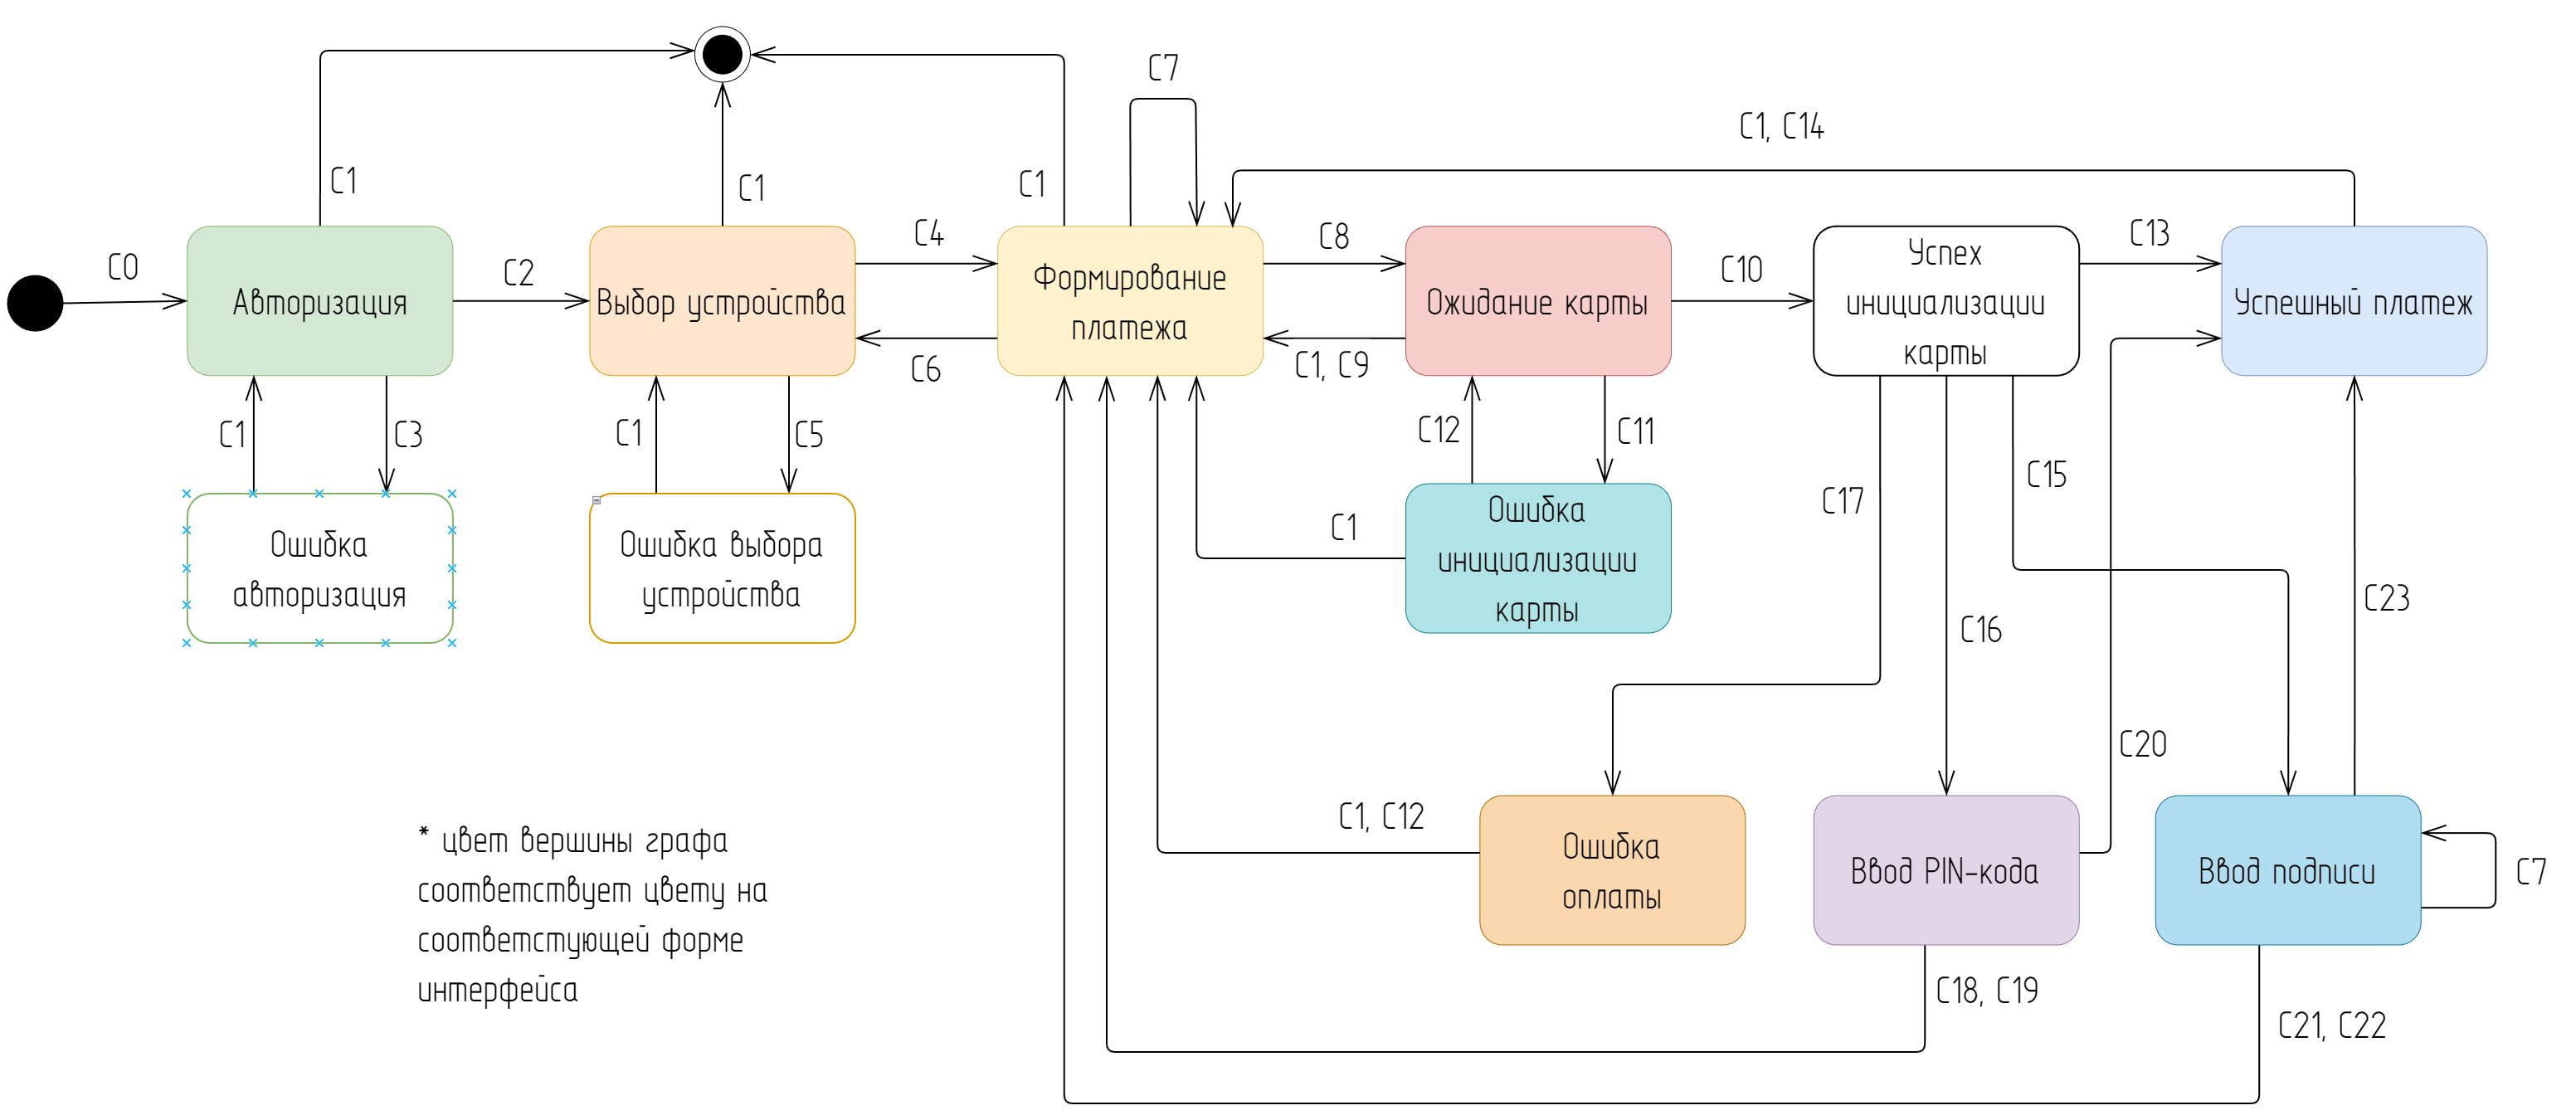
\includegraphics[width=1\textwidth]{images/design/nav_graph}
    \caption{\centering Граф состояний интерфейса}
    \label{fig:nav_graph}
\end{figure}

На котором введены следующие обозначения событий:
\begin{itemize}
    \item С0~--- открытие приложения,
    \item С1~--- нажатие системной кнопки <<Назад>>,
    \item С2~--- успешная авторизация после ввода данных и нажатия кнопки <<Войти>>,
    \item С3~--- ошибка авторизации после нажатия кнопки <<Войти>>,
    \item С4~--- успешное подключение к устройству после выбора устройства и нажатия <<Продолжить>>,
    \item С5~--- ошибка подключение к устройству после выбора устройства и нажатия <<Продолжить>>
    \item С6~--- нажатие иконки <<Настройки>>,
    \item С7~--- нажатие иконки <<Очистить данные>>,
    \item С8~--- нажатие кнопки <<Оплатить>>,
    \item С9~--- нажатие кнопки <<Отменить>>,
    \item С10~--- успешная инициализация карты,
    \item С11~--- ошибка при инициализации карты,
    \item С12~--- нажатие кнопки <<Повторить попытку>>,
    \item С13~--- успешное выполнение платежа,
    \item С14~--- нажатие кнопки <<Новый платеж>>,
    \item С15~--- запрос ввода подписи держателя карты,
    \item С16~--- запрос ввода PIN-кода держателя карты,
    \item С17~--- ошибка выполнения платежа,
    \item С18~--- ошибка проверки PIN-кода,
    \item С19~--- успешная проверка PIN-кода и ошибка при выполнении платежа,
    \item C20~--- успешная проверка PIN-кода и успешное выполнение платежа,
    \item С21~--- ошибка проверки подписи,
    \item С22~--- успешная проверка подписи и ошибка при выполнении платежа,
    \item С23~--- успешная проверка подписи и успешное выполнение платежа.
\end{itemize}


Для разрабатываемой программы была спроектирована диаграмма классов, показывающая особенности интеграции бизнес-логики и интерфейса экранов.
Диаграмма представлена на риснуке~\ref{fig:classes}.
На ней изображены классы модулей авторизации, подключения устройства-считывателя, выполнения платежа.

\begin{figure}[H]
    \centering
    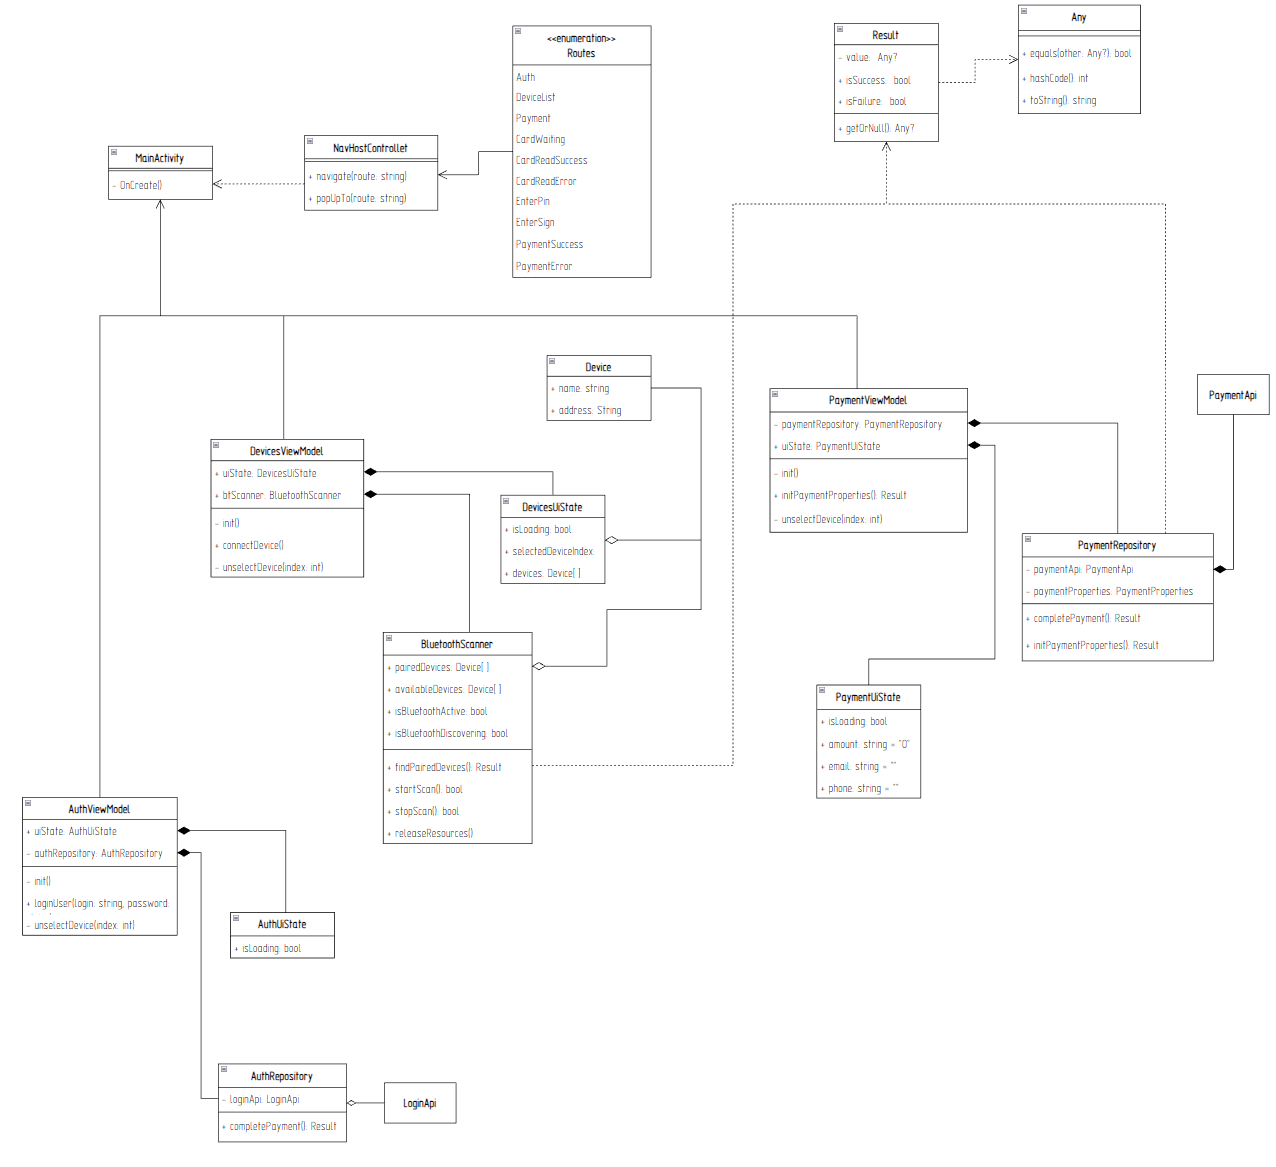
\includegraphics[angle=90, width=1\textwidth]{images/design/classes}
    \caption{\centering Диаграмма классов мобильного приложения}
    \label{fig:classes}
\end{figure}

Для разработанного приложения было проведено структурное тестирование методом покрытия операторов.
Выполнения тестовых случаев и их проверка осуществлялось с помощью библиотек Mockk и JUnit для структурного и модульного тестирования.
Описание тестовых случаев, проверяющих работу устройства, перечислено в таблице~\ref{tab:mob_app_test_cases}.

\begin{longtable}[l]{| P{0.18\textwidth} | P{0.2\textwidth} | P{0.26\textwidth} | P{0.26\textwidth}|}

    \caption{Тестовые случаи структурного тестирования программной части системы}
    \label{tab:mob_app_test_cases} \\
    \hline
    \textbf{Тестируемый модуль} &
    \textbf{Описание теста} &
    \textbf{Ожидаемый результат} &
    \textbf{Полученный результат} \\
    \hline
    \endfirsthead

    \caption*{Продолжение таблицы~\ref{tab:mob_app_test_cases}} \\
    \hline
    \textbf{Тестируемый модуль} &
    \textbf{Описание теста} &
    \textbf{Ожидаемый результат} &
    \textbf{Полученный результат} \\
    \hline
    \endhead

    \hline
    \endfoot

    \hline
    \endlastfoot

    Авторизация &
    Ввод корректных логина и пароля и нажатие кнопки <<Войти>> &
    Успешная авторизация, переход на экран выбора устройства &
    Успешная авторизация, переход выполнен \\
    \hline

    Авторизация &
    Ввод некорректных данных (неверный логин или пароль) &
    Отображение ошибки, очистка полей ввода &
    Сообщение об ошибке отображено, поля очищены \\
    \hline

    Выбор устройства &
    Проверка наличия доступных Bluetooth-устройств &
    Список устройств успешно заполнен, устройства обнаружены &
    Список устройств отобразился корректно \\
    \hline

    Выбор устройства &
    Выбор считывателя бесконтактных карт из списка &
    Подключение к устройству, подтверждение типа устройства &
    Устройство определено как считыватель карт \\
    \hline

    Выбор устройства &
    Нажатие на несовместимое устройство &
    Сообщение о невозможности подключения к данному устройству &
    Пользователь уведомлен о несовместимости \\
    \hline

    Создание платежа &
    Ввод корректной суммы, номера телефона и/или email для чека, нажатие <<Оплатить>> &
    Отправка запроса на инициализацию карты &
    Данные переданы, переход на следующий экран выполнен \\
    \hline

    Создание платежа &
    Ввод некорректной суммы (например, 0 или отрицательное число) &
    Подсветка поля ввода, вывод сообщения об ошибке &
    Поле выделено, ошибка отображена \\
    \hline

    Инициализация карты &
    Поднесение бесконтактной карты к считывателю &
    Успешная инициализация карты, получение данных от неё &
    Карта распознана, данные получены \\
    \hline

    Инициализация карты &
    Поднесение несовместимого устройства или его отсутствие &
    Переход на экран ошибки инициализации карты &
    Экран ошибки отображен, есть возможность повторить попытку \\
    \hline

    Ввод PIN-кода &
    Запрос на ввод PIN-кода со стороны карты &
    Открытие экрана ввода PIN, отправка кода через REST API &
    Экран ввода отображен, данные переданы на сервер \\
    \hline

    Ввод PIN-кода &
    Ввод неверного PIN более трёх раз &
    Блокировка карты, переход на экран ошибки &
    Карта заблокирована, транзакция прервана \\
    \hline

    Ввод подписи &
    Запрос на ввод подписи держателя карты &
    Открытие экрана ввода подписи, отправка данных на сервер &
    Экран отображен, данные отправлены \\
    \hline

    Ввод подписи &
    Отказ пользователя от ввода подписи &
    Отмена транзакции по сигналу сервера &
    Транзакция отменена, переход на экран ошибки \\
    \hline

    Успех/ошибка платежа &
    Получение положительного ответа от банка &
    Отображение экрана успешной транзакции с данными о платеже &
    Экран успеха отображен, информация о платеже корректна \\
    \hline

    Успех/ошибка платежа &
    Получение отрицательного ответа от банка &
    Отображение экрана ошибки с причиной, возможность начать новую транзакцию &
    Экран ошибки отображен, можно создать новую транзакцию \\
    \hline

    Все модули &
    Обрыв связи с терминалом во время транзакции &
    Отображение ошибки связи, возможность повторного подключения &
    Ошибка связи отображена, можно повторить попытку \\
    \hline
\end{longtable}


Тестирование устройства также проводилось методом покрытия операторов.
Оно представляет собой отдельную версию программного обеспечения МК, содержащую только код тестов, расположенных в директории test исходного проекта. 
Результатом тетсирования является загрузка данного ПО на МК с выполнением всех тестов и выводом отладочных сообщений.
Значения в таблице~\ref{tab:test_cases_hardware} показывают корректность работы програмнного обеспечения МК.

\begin{longtable}[l]{| P{0.18\textwidth} | P{0.2\textwidth} | P{0.26\textwidth} | P{0.26\textwidth}|}

    \caption{Тестовые случаи структурного тестирования аппаратной части системы}
    \label{tab:test_cases_hardware} \\
    \hline
    \textbf{Тестируемый модуль} &
    \textbf{Описание теста} &
    \textbf{Ожидаемый результат} &
    \textbf{Полученный результат} \\
    \hline
    \endfirsthead

    \caption*{Продолжение таблицы~\ref{tab:test_cases_hardware}} \\
    \hline
    \textbf{Тестируемый модуль} &
    \textbf{Описание теста} &
    \textbf{Ожидаемый результат} &
    \textbf{Полученный результат} \\
    \hline
    \endhead

    \hline
    \endfoot

    \hline
    \endlastfoot

    Подключение по Bluetooth &
    Включение Bluetooth на устройстве и попытка подключения к терминалу &
    Установление устойчивого соединения между смартфоном и считывателем &
    Подключение выполнено успешно \\
    \hline

    Передача данных по Bluetooth &
    Отправка команды от приложения к терминалу через Bluetooth &
    Команда корректно передана и обработана терминалом &
    Данные получены и обработаны \\
    \hline

    Получение данных по Bluetooth &
    Прием ответа от терминала после выполнения команды &
    Приложение получает данные в корректном формате &
    Данные успешно получены и интерпретированы \\
    \hline

    Активация Bluetooth-модуля &
    Проверка наличия и активации Bluetooth-адаптера на считывателе &
    Модуль Bluetooth должен быть готов к подключению и сканированию &
    Bluetooth-модуль активирован \\
    \hline

    Активация NFC-модуля &
    Активация NFC-чипа для чтения карты &
    NFC-модуль должен быть активен и готов к работе &
    NFC-модуль успешно активирован \\
    \hline

    Получение UID карты (ISO/IEC 14443-3) &
    Поднесение бесконтактной карты к считывателю &
    Считыватель определяет идентификатор карты (UID) в соответствии с протоколом ISO/IEC 14443-3 &
    UID успешно считан и передан в приложение \\
    \hline

    Активация карты (ISO/IEC 14443-4) &
    Инициализация протокола транспортного уровня с картой &
    Установлено логическое соединение с картой, карта готова к обмену APDU-командами &
    Карта успешно активирована \\
    \hline

    Обмен APDU-командами &
    Отправка команд SELECT AID, GET PROCESSING OPTIONS &
    Карта корректно отвечает на APDU-запросы &
    APDU-обмен прошел успешно \\
    \hline

    Чтение данных с карты &
    Запрос данных о платежном приложении (например, AID, номере карты) &
    Данные успешно прочитаны и переданы в мобильное приложение &
    Данные получены корректно \\
    \hline

    Генерация криптограммы &
    Выполнение команды GENERATE AC &
    Карта генерирует Application Cryptogram, который передается в приложение &
    Криптограмма получена и передана в банк \\
    \hline

    Защита данных &
    Попытка несанкционированного доступа к данным карты через NFC-сниффинг &
    Система не должна позволять получить конфиденциальные данные без авторизации &
    Данные защищены, доступ невозможен \\
    \hline

    Ошибки связи &
    Разрыв Bluetooth-соединения во время транзакции &
    Приложение должно уведомить пользователя, операция будет отменена &
    Связь разорвана, транзакция отменена \\
    \hline

    Обработка ошибок NFC &
    Некорректная или поврежденная карта находится в поле считывателя &
    Считыватель должен распознать ошибку и сообщить пользователю &
    Ошибка обнаружена, выводится сообщение \\
    \hline

    Совместимость с картами ПС МИР &
    Поддержка работы с картой платёжной системы МИР &
    Устройство должно корректно работать со всеми совместимыми картами &
    Все тестовые карты успешно прошли инициализацию \\
    \hline

\end{longtable}

Тестирование интеграции частей системы проводилось в соответствии с описанием в подразделе~\ref{subsec:test_integr} ручным способом.
Для начала была протестирована реакция системы на поднесение бесконтактной платежный карты к NFC-модулю.
Если карта обнаруживалась и распознавалась корректно, то устройство выводило текст, информирующий об успешной идентификации карты и её уникальный идентификатор UID.
В случае возникновения ошибки на последовательный порт отправлялись сообщения с описанием проблемы, множественный вывод в различных местах позволял определять причину неисправности.

Для проверки работоспособности системы производились примитивные тесты.
Проверка корректной работы:
\begin{enumerate}
    \item поднесена карта с поддержкой стандарта устройства;
    \item ожидаемая реакция: успешное считывание и идентификация;
    \item полученный результат: успешное считывание.
\end{enumerate}

Проверка некорректного работы:
\begin{enumerate}
    \item поднесены неподдерживаемая карта;
    \item ожидаемая реакция: отсутствие реакции NFC-модуля;
    \item полученный результат: стандартный цикл использования устройства без взаимодействия с предметом/картой.
\end{enumerate}

На рисунке ~\ref{fig:test_success} показаны данные на Serial Monitor при успешной работе системы.

\begin{figure}[H]
    \centering
    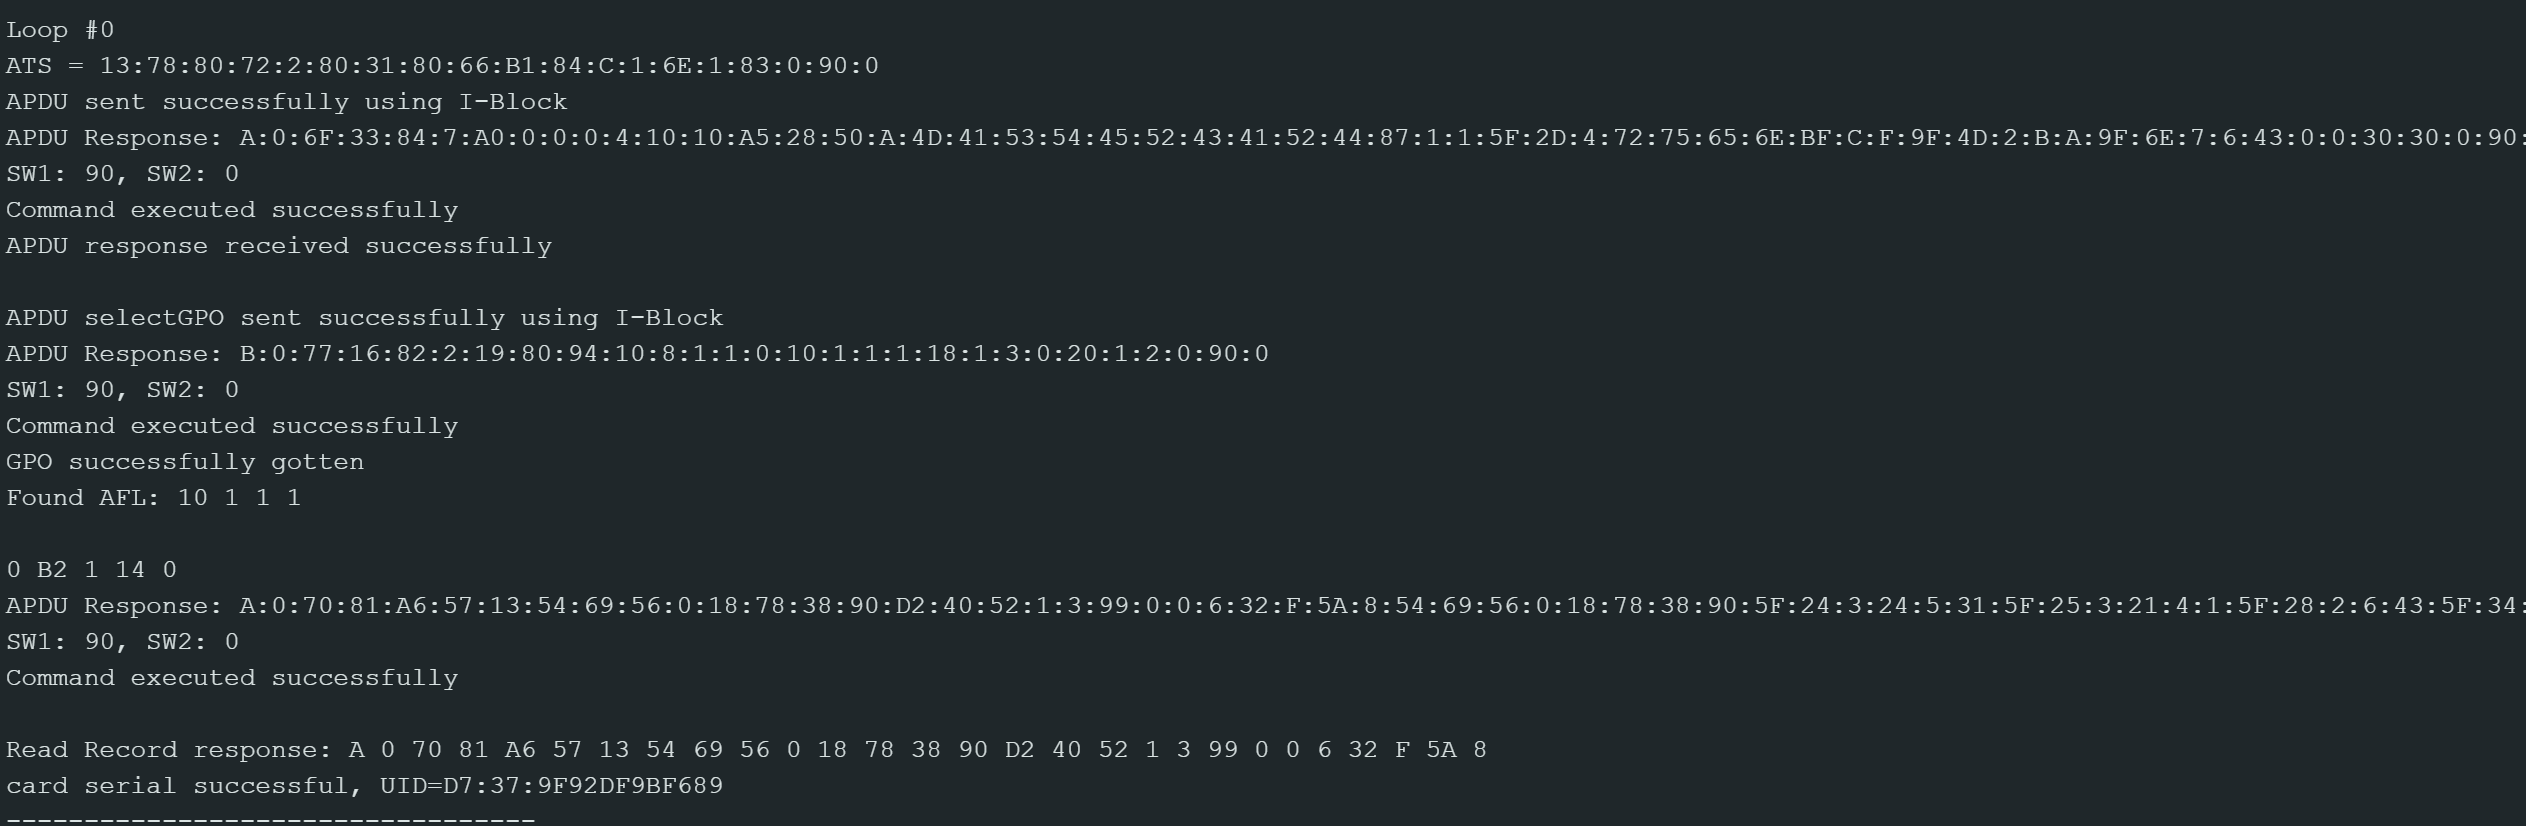
\includegraphics[width=0.9\textwidth]{images/design/test_success}
    \caption{\centering Резльтат успешного тестирования системы}
    \label{fig:test_success}
\end{figure}
